 

\cell
W bieżącym rozdziale szczegółowo opisany zostanie proces tworzenia autorskiej głębokiej sieci neuronowej o nazwie $\textit{GML-Net}$. Sieć ta została skonstruowana przez autora niniejszej pracy w celu przeprowadzenia efektywnej detekcji budynków na zdjęciach lotniczych pochodzących ze zbioru $\textit{Inria Aerial Image Labeling Dataset}$. W pierwszej części rozdziału przedstawione zostaną najważniejsze hiperparametry modelu oraz proces wczytywania, podziału i obróbki danych treningowych i walidacyjnych. W kolejnej części przedstawiona zostanie architektura sieci \textit{GML-Net}, warstwy przetwarzania (bloki), które tę architekturę tworzą oraz sposób trenowania tej sieci.

\vspace{-0.5cm}
\cell
\ss{ Najważniejsze hiperparametry sieci}

\cell
Pierwszym krokiem procesu tworzenia modelu finalnej sieci neuronowej jest definicja bibliotek języka Python, które zostaną wykorzystane w trakcie obliczeń na poszczególnych etapach tworzenia modelu. Główną biblioteką, która została zastosowana w bieżącej pracy do implementacji głębokiego uczenia jest biblioteka $\textit{PyTorch}$. Została ona wybrana, gdyż pozwala ona na efektywne i elastyczne posługiwanie się podstawowymi jednostkami przetwarzania w architekturze głębokich sieci neuronowych, zapewnia pełną integrację z~biblioteką $\textit{NumPy}$ oraz umożliwia wygodną definicję zbiorów danych uczących i~walidacyjnych.
\vspace{0.5cm}

\cell
\begin{lstlisting}[name=Rozdzial3.1, language=Python]
import os
import time
import copy
import glob
import torch
import random
import numpy as np
import pandas as pd
from math import exp
from PIL import Image
import torch.nn as nn
import torch.optim as optim
from datetime import datetime
from google.colab import drive
import matplotlib.pyplot as plt
from torchsummary import summary
from torch.utils.data import Dataset
from torchvision import transforms, models
from numpy.lib.stride_tricks import as_strided
from collections import defaultdict, OrderedDict
\end{lstlisting}


\cell
Kolejnym krokiem tworzenia sieci $\textit{GML-Net}$ była definicja jej najważniejszych hiperparametrów, którymi są:
\begin{itemize}
  \item rozdzielczość fragmentów obrazów, na których trenowana będzie sieć $\textit{GML-Net}$ ($\textit{sample$\_$res}$), 
  \item rozdzielczość obrazów na jakie będzie podzielony zostanie obraz wejściowy przed pobraniem z niego próbek $\textit{sample$\_$res}$ x $\textit{sample$\_$res}$ ($\textit{sub$\_$arr$\_$size}$),
  \item rozmiar batcha w data loaderze ($\textit{batch$\_$s}$),
  \item najważniejsze parametry optymalizatora ($\textit{learn$\_$rate}$, $\textit{momt}$, $\textit{wght$\_$dec}$),
  \item najważniejsze parametry schedulera ($\textit{step$\_$s}$, $\textit{gamm}$),
  \item wagi poszczególnych składowych funkcji strat ($\textit{wghts$\_$dict}$),
  \item wartość, powyżej której uznajemy że dany piksel został zakwalifikowany jako będący częścią budynku ($\textit{loss$\_$thres}$),
  \item liczba epok trenowania ($\textit{epoch$\_$num}$),
  \item minimalna wartość stopy uczenia ($\textit{optim$\_$eps}$). 
\end{itemize}
\vspace{1cm}

\cell
\begin{lstlisting}[name=Rozdzial3.1, language=Python]
google_path = "/content/drive/My Drive/GSN/Thesis/Dane/AID/"
train_path = "/content/AerialImageDataset/"
mdl_path = "/content/drive/My Drive/GSN/Thesis/Najlepszy model/"
mdl_name = "ResNet50_wide_UNet_depth_3_BottleNeck_BS_18"
org_h_dim = 5000
org_v_dim = 5000
sub_arr_size = 1000
sample_res = 256
recalc_flag = False
batch_s = 18
learn_rate = 0.01
momt = 0.9
wght_dec = 0.0005
step_s = 5
gamm = 0.5
wghts_dict = {"bce": 0.3, "lhl": 0.3, "dice": 0.4}
loss_thres = 0.5
epoch_num = 200
optim_eps = 1e-08
\end{lstlisting}


\cell
Jak widać wartości zastosowanych hiperparamterów sieci $\textit{GML-Net}$ w dużej części pokrywają się z wartościami hiperparapetrów obserwowanych w literaturze badawczej - zdecydowano się na obrazy o rozdzielczości $\textit{256x256}$ pikseli, początkową stopę uczenia na poziomie 0,01, momentum wartości 0,9 i spadek wag równy 0,0005.

\cell
\begin{lstlisting}[name=Rozdzial3.1, language=Python]
params_dict = {}
params_dict["sub_arr_size"] = sub_arr_size
params_dict["sample_res"] = sample_res
params_dict["recalc_flag"] = recalc_flag
params_dict["batch_s"] = batch_s
params_dict["learn_rate"] = learn_rate
params_dict["momt"] = momt
params_dict["wght_dec"] = wght_dec
params_dict["step_s"] = step_s
params_dict["gamm"] = gamm
params_dict["bce"] = wghts_dict["bce"]
params_dict["lhl"] = wghts_dict["lhl"]
params_dict["dice"] = wghts_dict["dice"]
params_dict["loss_thres"] = loss_thres
params_dict["epoch_num"] = epoch_num
params_dict["org_h_dim"] = org_h_dim
params_dict["org_v_dim"] = org_v_dim
\end{lstlisting}


\cell
Wartości wszystkich hiperparmetrów modelu zostały zapisane w słowniku $\textit{params$\_$dict}$, po to by zawsze mieć pewność przy użyciu jakich hiperparametrów dany model był trenowany.

\vspace{-0.5cm}
\cell
\ss{ Dane uczące i ich transformacje}

\cell
Pierwszym krokiem przygotowania danych treningowych i walidacyjnych sieci $\textit{GML-Net}$ był import zbioru treningowego $\textit{Inria Aerial Image Labeling Dataset}$ z dysku  $\textit{Google}$ na dysk  $\textit{Coloba}$.
\vspace{1cm}

\cell
\begin{lstlisting}[name=Rozdzial3.1, language=Python]
drive.mount('/content/drive')

if os.path.exists("sample_data"):
  !rm -r sample_data

if not os.path.exists(train_path):
  !cp -R "$google_path" $train_path

curr_wd = os.getcwd()
\end{lstlisting}


\cell
Pobrany zbiór treningowy składa się ze 180 zdjęć lotniczych pięciu miast: Austin, Chicago, Hrabstwo Kitsap, Tyrol oraz Wiedeń - po 36 zdjęć każdego z miast. Każde z tych zdjęć ma przypisaną do siebie maskę $\textit{ground truth}$, która wskazuje które piksele zdjęcia bazowego reprezentują budynki. Zdjęcia bazowe mają rozdzielczość $\textit{5000x5000}$ pikseli, trzy kanały przestrzenne, każde z nich pokrywa teren o powierzchni $\textit{1500x1500}$ m$^2$. Zbiór walidacyjny został wydzielony ze zbioru treningowego poprzez wybranie pięciu pierwszych zdjęć każdego z miast (zgodnie z podejściem zastosowanym w literaturze badawczej) - w ten sposób powstał finalny zbiór treningowy składający się ze 155 zdjęć oraz finalny zbiór walidacyjny składający się z 25 zdjęć. Opisany tu podział jest realizowany przy pomocy funkcji $\textit{create$\_$meta$\_$info}$, która tworzy pliki  $\textit{CSV}$ zawierające ścieżki do zdjęć z poszczególnych zbiorów. 

\cell
\begin{lstlisting}[name=Rozdzial3.1, language=Python]
def create_meta_info(root_directory):    
  l_meta = [] 
  l_meta_t = []
  l_meta_v = []
  os.chdir(root_directory)

  for file in glob.glob("*_GT.tif"):
    mask_path = os.path.join(root_directory, file)
    im_path = os.path.join(root_directory, file[:-7] + ".tif")
    l_meta.append((im_path, mask_path))
    if not im_path[-6].isdigit() and im_path[-5] in ["1", "2", "3", "4", "5"]:
      l_meta_v.append((im_path, mask_path))
    else:
      l_meta_t.append((im_path, mask_path))

  os.chdir(curr_wd)
  if l_meta:
    pd.DataFrame(l_meta).to_csv('m_inf.csv', index=False, header=False)
    pd.DataFrame(l_meta_t).to_csv('m_inf_t.csv', index=False, header=False)
    pd.DataFrame(l_meta_v).to_csv('m_inf_v.csv', index=False, header=False)
\end{lstlisting}


\cell
Posiadając już zdjęcia podzielone na zbiór treningowy i walidacyjny, kolejnym etapem obróbki danych było wydzielenie odpowiednich próbek z tych zdjęć. W związku z tym, iż zbiór $\textit{Inria Aerial Image Labeling Dataset}$ składa się ze zdjęć o bardzo wysokiej rozdzielczości i niemożliwe oraz bardzo nieefektywne byłoby przeprowadzenie treningu sieci neuronowej na zdjęciach o rozdzielczości $\textit{5000x5000}$ zdecydowano się na podział tych zdjęć (oraz odpowiadających im masek) na 25 równych części, każda o rozdzielczości 1000x1000 pikseli. Dodatkowo, żeby nie utracić informacji znajdujących się na krawędziach podzielonych zdjęć, ze zdjęć bazowych (oraz z odpowiadających im masek) zdecydowano sie wydzielić kolejnych 16 części (również o rozdzielczości $\textit{1000x1000}$ pikseli) znajdujących się na łączeniach każdych czterech sąsiadujących ze sobą bazowych części. W ten sposób z każdego zdjęcia znajdującego się w bazowym zbiorze treningowym pozyskano 41 fragmentów (oraz 41 fragmentów odpowiadających im masek), co przekłada się na łączną liczbę 6355 fragmentów trenujących (155 * 41). Dodając do tego fakt, iż z~każdego takiego fragmentu wybranych zostanie 18 losowych okien (rozmiar partii równy 18) o rozmiarach $\textit{256x256}$ pikseli, uzyskujemy finalnie 114390 przykładów uczących. Pobieranie fragmentów z poszczególnych zdjęć (masek) zostało zrealizowane przy pomocy funkcji $\textit{resample}$, która z kolei opiera się na funkcji $\textit{as$\_$strided}$ pochodzącej z biblioteki $\textit{numpy.lib.stride$\_$tricks}$.

\cell
\begin{lstlisting}[name=Rozdzial3.1, language=Python]
def resample(image, N, org_h_dim, org_v_dim):
  wind_h = wind_w = N
  img_shp = image.shape
  nm_cls = img_shp[-1] if len(img_shp) > 2 else 1
  n_arrs1 = int((img_shp[0] // wind_h))
  n_arrs2 = int((img_shp[1] // wind_w))
  s_l = wind_h * org_h_dim * nm_cls
  s_k = wind_w * nm_cls

  if nm_cls == 1:
    new_strds = (s_l, s_k, org_v_dim * nm_cls, nm_cls)
    new_shape = (n_arrs1, n_arrs2, wind_h, wind_w)
    img_winds = as_strided(image, shape=new_shape, strides=new_strds)
    fin_winds = img_winds.reshape((n_arrs1 * n_arrs2, wind_h, wind_w))
  else:
    new_strds = (s_l, s_k, org_v_dim * nm_cls, nm_cls, 1)
    new_shape = (n_arrs1, n_arrs2, wind_h, wind_w, nm_cls)
    img_winds = as_strided(image, shape=new_shape, strides=new_strds)
    fin_winds = img_winds.reshape((n_arrs1*n_arrs2, wind_h, wind_w, nm_cls))
  return fin_winds
\end{lstlisting}


\cell
Pozyskane fragmenty zdjęć i masek zostały następnie połączone w listy, w celu ułatwienia ich przetwarzania na kolejnych etapach - łączenie to zostało zrealizowane przy pomocy funkcji $\textit{get$\_$img$\_$smpl}$.

\cell
\begin{lstlisting}[name=Rozdzial3.1, language=Python]
def get_img_smpl(idx, sub_arr_size, img_arr, org_h_dim, org_v_dim):
  image = np.array(Image.open(img_arr[idx, 0]))
  mask = np.array(Image.open(img_arr[idx, 1]))
  img_sub_arrs1 = resample(image, sub_arr_size, org_h_dim, org_v_dim)
  msk_sub_arrs1 = resample(mask, sub_arr_size, org_h_dim, org_v_dim)
  s1 = list(zip(img_sub_arrs1, msk_sub_arrs1))
  half_wind = int(sub_arr_size // 2)
  img_hv = image[half_wind:-half_wind, half_wind:-half_wind, ...]
  mask_hv = mask[half_wind:-half_wind, half_wind:-half_wind, ...]
  img_sub_arrs2 = resample(img_hv, sub_arr_size, org_h_dim, org_v_dim)
  msk_sub_arrs2= resample(mask_hv, sub_arr_size, org_h_dim, org_v_dim)
  s2 = list(zip(img_sub_arrs2, msk_sub_arrs2))
  return s1, s2
\end{lstlisting}


\cell
Aby ułatwić proces pobierania fragmentów ze zdjęć i masek bazowych oraz umożliwić ich efektywną augmentację postanowiono połączyć te operacje przy pomocy jednej klasy $\textit{ResampledImageDataset}$.

\cell
\begin{lstlisting}[name=Rozdzial3.1, language=Python]
class ResampledImageDataset(Dataset):
  def __init__(self, csv_file, org_h, org_v, sub_arr_s, transform=None):
    self.img_arr = pd.read_csv(csv_file, header=None).values
    self.trasform = transform
    self.org_h = org_h
    self.org_v = org_v
    self.sub_arr_s = sub_arr_s

  def __len__(self):
    return len(self.img_arr)

  def __getitem__(self, idx):
    s1, s2 = get_img_smpl(idx, self.sub_arr_s, self.img_arr, self.org_h, 
                          self.org_v)   

    if self.trasform is not None:
      s1 = self.trasform(s1)
      s2 = self.trasform(s2)   
    return s1 + s2
\end{lstlisting}


\cell
Dodatkowo, aby wyliczyć średnią i odchylenie standardowe dla poszczególnych kanałów zdjęć bazowych po to by móc zastosować te statystyki do normalizacji, stworzono klasę $\textit{BasicImageDataset}$.

\cell
\begin{lstlisting}[name=Rozdzial3.1, language=Python]
class BasicImageDataset(Dataset):
  def __init__(self, csv_file, transform=None):
    self.images_arr = pd.read_csv(csv_file, header=None).values
    self.trasform = transform

  def __len__(self):
    return len(self.images_arr)

  def __getitem__(self, idx):
    image = np.array(Image.open(self.images_arr[idx, 0]))
    mask = np.array(Image.open(self.images_arr[idx, 1]))
    sample = [image, mask]

    if self.trasform is not None:
      sample = self.trasform(sample)
    
    return sample
\end{lstlisting}


\cell
Dla każdego zdjęcia pochodzącego z klasy $\textit{BasicImageDataset}$ zapisywane są wartości jego kolorów w poszczególnych kanałach, a po przejściu przez wszystkie zdjęcia wyliczane są globalne średnie i odchylenia standardowe dla wszystkich kanałów.

\cell
\begin{lstlisting}[name=Rozdzial3.1, language=Python]
create_meta_info(train_path)
basic_ds = BasicImageDataset("m_inf.csv")
basic_ds_len = len(basic_ds)
sngl_img_pxl_num = basic_ds[0][0].size
tot_pxl_num = (sngl_img_pxl_num * basic_ds_len) / 3

if recalc_flag:
  mean_rgbs = (np.array([sample[0].sum((0, 1)) for sample in 
                        basic_ds]).sum(0) / tot_pxl_num) / 255
  std_rgbs = np.sqrt(np.array([np.power(sample[0] - mean_rgbs, 2).sum((0, 1)) 
                                        for sample in basic_ds]).sum(0) / 
                                        tot_pxl_num) / 255
else:
  mean_rgbs = np.array([0.40483995, 0.42726254, 0.39271341])
  std_rgbs = np.array([0.45071778, 0.4634665 , 0.42900409])
\end{lstlisting}


\cell
Kolejnym etapem tworzenia zbiorów treningowego i walidacyjnego jest definicja augmentacji, które zostaną zastosowane na tych zbiorach.

\cell
\begin{lstlisting}[name=Rozdzial3.1, language=Python]
class RandomHorizontalFlip(object):
  def __init__(self, p=0.5):
    super().__init__()
    self.p = p
  
  def __call__(self, all_samples):
    trans_list = []

    for sample in all_samples:
      image, mask = sample[0], sample[1]
      image = transforms.functional.to_pil_image(image)
      mask = transforms.functional.to_pil_image(mask)

      if torch.rand(1) < self.p:
        image = transforms.functional.hflip(image)
        mask = transforms.functional.hflip(mask)

      trans_list.append((image, mask))

    return trans_list
\end{lstlisting}


\cell
Pierwszą z nich jest augmentacja realizowana przez losowy horyzontalny obrót zdjęcia (maski) wzdłuż środkowej osi - losowość polega na tym, iż taka augmentacja dochodzi do skutku z prawdopodobieństwem 50$\%$ - czyli dla co drugiego zdjęcia.

\cell
\begin{lstlisting}[name=Rozdzial3.1, language=Python]
class RandomVerticalFlip(object):
  def __init__(self, p=0.5):
    super().__init__()
    self.p = p
  
  def __call__(self, all_samples):
    trans_list = []

    for sample in all_samples:
      image, mask = sample[0], sample[1]

      if torch.rand(1) < self.p:
        image = transforms.functional.vflip(image)
        mask = transforms.functional.vflip(mask)

      trans_list.append((image, mask))

    return trans_list
\end{lstlisting}


\cell
Drugą zdefiniowaną augmentacją jest losowy wertykalny obrót zdjęcia (maski) wzdłuż środkowej osi, który również jest realizowany z prawdopodobieństwem 50$\%$.

\cell
\begin{lstlisting}[name=Rozdzial3.1, language=Python]
class RandomRotation(object):
  def __call__(self, all_samples):

    trans_list = []

    for sample in all_samples:
      image, mask = sample[0], sample[1]
      angle_mult = random.randint(0, 12)
      rot_img = transforms.functional.rotate(image, angle_mult * 30, expand=True)
      rot_mask = transforms.functional.rotate(mask, angle_mult * 30, expand=True)
      trans_list.append((rot_img, rot_mask))
    
    return trans_list
\end{lstlisting}


\cell
Kolejną augmentacją zdefiniowaną dla zbiorów treningowego i walidacyjnego jest rotacja zdjęcia (maski) o losowy kąt będący wielokrotnością kąta 30 stopni.

\cell
\begin{lstlisting}[name=Rozdzial3.1, language=Python]
class RandomCrop(object):
  def __init__(self, out_s):
    assert isinstance(out_s, (int, tuple))
    self.out_s = out_s     

  def __call__(self, all_samples):
    trans_list = []

    for sample in all_samples:
      image, mask = np.array(sample[0]), np.array(sample[1])
      out_s = (self.out_s, self.out_s) if isinstance(self.out_s, int) else out_s
      new_h, new_w = out_s
      top = np.random.randint(0, image.shape[0] - new_h)
      left = np.random.randint(0, image.shape[1] - new_w)
      image = image[top:(top + new_h), left: left + new_w]
      mask = mask[top:(top + new_h), left: left + new_w]
      trans_list.append((image, mask))
    
    return trans_list
\end{lstlisting}


\cell
Następną augmentacją wykorzystywaną przy budowie sieci $\textit{GML-Net}$ jest wybór losowego okna o rozmiarach $\textit{256x256}$ pikseli. 

\cell
\begin{lstlisting}[name=Rozdzial3.1, language=Python]
 class Normalize(object):    
  def __init__(self, mean, std, inplace=False):
    self.mean = mean
    self.std = std
    self.inplace = inplace
  
  def __call__(self, all_samples):
    trans_list = []

    for sample in all_samples:
      image, mask = sample[0], sample[1]
      norm_img = transforms.functional.normalize(image / 255.0, self.mean, 
                                                self.std, self.inplace)
                                                
      norm_mask = mask / 255.0
      trans_list.append((norm_img, norm_mask))
    
    return trans_list
\end{lstlisting}


\cell
Ostatnią augmentacją wykorzystywaną w bieżącej pracy jest normalizacja zdjęć przy użyciu globalnych średnich i odchyleń standardowych, których sposób wyliczenia został opisany powyżej.
\vspace{0.5cm}

\cell
\begin{lstlisting}[name=Rozdzial3.1, language=Python]
class ToTensor(object):
  def __call__(self, all_samples):

    trans_list = []

    for sample in all_samples:
      image, mask = np.array(sample[0]), np.array(sample[1])
      trans_list.append((torch.from_numpy(image).permute(2, 0, 1), 
                          torch.from_numpy(mask)))
    return trans_list
\end{lstlisting}


\cell
Po zastosowaniu wszystkich augmentacji, należy przekonwertować zdjęcia (maski) z~formatu macierzy $\textit{NumPy}$ do formatu tensora $\textit{PyTorch}$ tak, żeby mogły one być wykorzystane do trenowania finalnej sieci neuronowej - odpowiedzialną za ten proces jest klasa $\textit{ToTensor}$.

\cell
\begin{lstlisting}[name=Rozdzial3.1, language=Python]
trn_trans = transforms.Compose([RandomHorizontalFlip(), 
                                RandomVerticalFlip(),
                                RandomRotation(), 
                                RandomCrop(sample_res), 
                                ToTensor(), 
                                Normalize(mean_rgbs, std_rgbs)])

train_dataset = ResampledImageDataset("m_inf_t.csv", org_h_dim, 
                                      org_v_dim, sub_arr_size, 
                                      transform=trn_trans)

vld_trans = transforms.Compose([RandomCrop(sample_res), ToTensor(), 
                                Normalize(mean_rgbs, std_rgbs)])
                                
valid_dataset = ResampledImageDataset("m_inf_v.csv", org_h_dim, 
                                      org_v_dim, sub_arr_size, 
                                      transform=vld_trans)
\end{lstlisting}


\cell
Finalnym krokiem tworzenia zbiorów treningowego i walidacyjnego było zdefiniowanie kolejności poszczególnych augmentacji. Jak widać w przypadku zbioru walidacyjnego augmentacje zostały ograniczone do wyboru losowego okna i normalizacji, po to by móc oceniać jakość modelu na jak najbardziej stabilnych danych.
\vspace{0.5cm}

\cell
\begin{lstlisting}[name=Rozdzial3.1, language=Python]
org_data_set = ResampledImageDataset("m_inf.csv", org_h_dim, 
                                     org_v_dim, sub_arr_size)
ds_len = len(org_data_set)
rnd_idx = random.randint(0, ds_len - 1)
rnd_idx2 = random.randint(0, len(org_data_set[0]) - 1)
org_img0, org_mask0 = org_data_set[rnd_idx][rnd_idx2]

org_img0_shp = org_img0.shape
org_img = np.zeros((org_img0_shp[0], org_img0_shp[1], 4), dtype=np.uint8)
org_img[..., :3] = org_img0
org_img[..., 3] = 255

plt_org_mask = np.zeros((org_img0_shp[0], org_img0_shp[1], 4), 
                        dtype=np.uint8)
plt_org_mask[..., 0] = org_mask0.squeeze()
plt_org_mask[org_mask0.squeeze() > 0, 3] = 180 
\end{lstlisting}


\cell
Kolejnym etapem obróbki i wczytywania danych było wyświetlenie losowego zdjęcia wraz z jego maską za zbioru treningowego po to by sprawdzić czy proces generowania danych uczących przebiega poprawnie.

\cell
\begin{lstlisting}[name=Rozdzial3.1, language=Python]
ds_len2 = len(train_dataset)
rnd_idx21 = random.randint(0, ds_len2 - 1)
rnd_idx22 = random.randint(0, len(train_dataset[0]) - 1)
trans_img0, trans_mask0 = train_dataset[rnd_idx21][rnd_idx22]

trans_img0 = torch.clamp(trans_img0, 0, 1).permute(1, 2, 0).cpu().numpy()
trans_img0_shp = trans_img0.shape
trans_img = np.zeros((trans_img0_shp[0], trans_img0_shp[1], 4))
trans_img[..., :3] = trans_img0
trans_img[..., 3] = 1.0

trans_mask0 = torch.clamp(trans_mask0, 0, 1).cpu().numpy()
plt_trans_mask = np.zeros((trans_img0_shp[0], trans_img0_shp[1], 4))
plt_trans_mask[..., 0] = trans_mask0.squeeze()
plt_trans_mask[trans_mask0.squeeze() > 0.5, 3] = 0.7
\end{lstlisting}


\cell
Aby móc efektywnie wyświetlić zdjęcie uczące wraz z odpowiadającą mu maską, zdecydowano się przekonwertować je do formatu RBGA po to by następnie móc je zwizualizować przy pomocy funkcji $\textit{plt}$ z biblioteki $\textit{matplotlib.pyplot}$.

\cell
\begin{lstlisting}[name=Rozdzial3.1, language=Python]
f2, axarr2 = plt.subplots(nrows=1, ncols=2, figsize=(20, 30))
axarr2[0].set_title("Oryginalne zdjecie\n", color='black', fontweight="bold",
                    fontsize=25)
axarr2[0].imshow(org_img)
axarr2[0].imshow(plt_org_mask, alpha=0.6)
axarr2[0].axis('off')
axarr2[1].imshow(trans_img)
axarr2[1].imshow(plt_trans_mask, alpha=0.6)
axarr2[1].axis('off')
axarr2[1].set_title("Przetransformowane zdjecie\n", color='black', 
                    fontweight="bold", fontsize=25)
plt.savefig('Org_trans_img.png', dpi=300, bbox_inches='tight')
\end{lstlisting}

\begin{figure}[!h]
    \centering 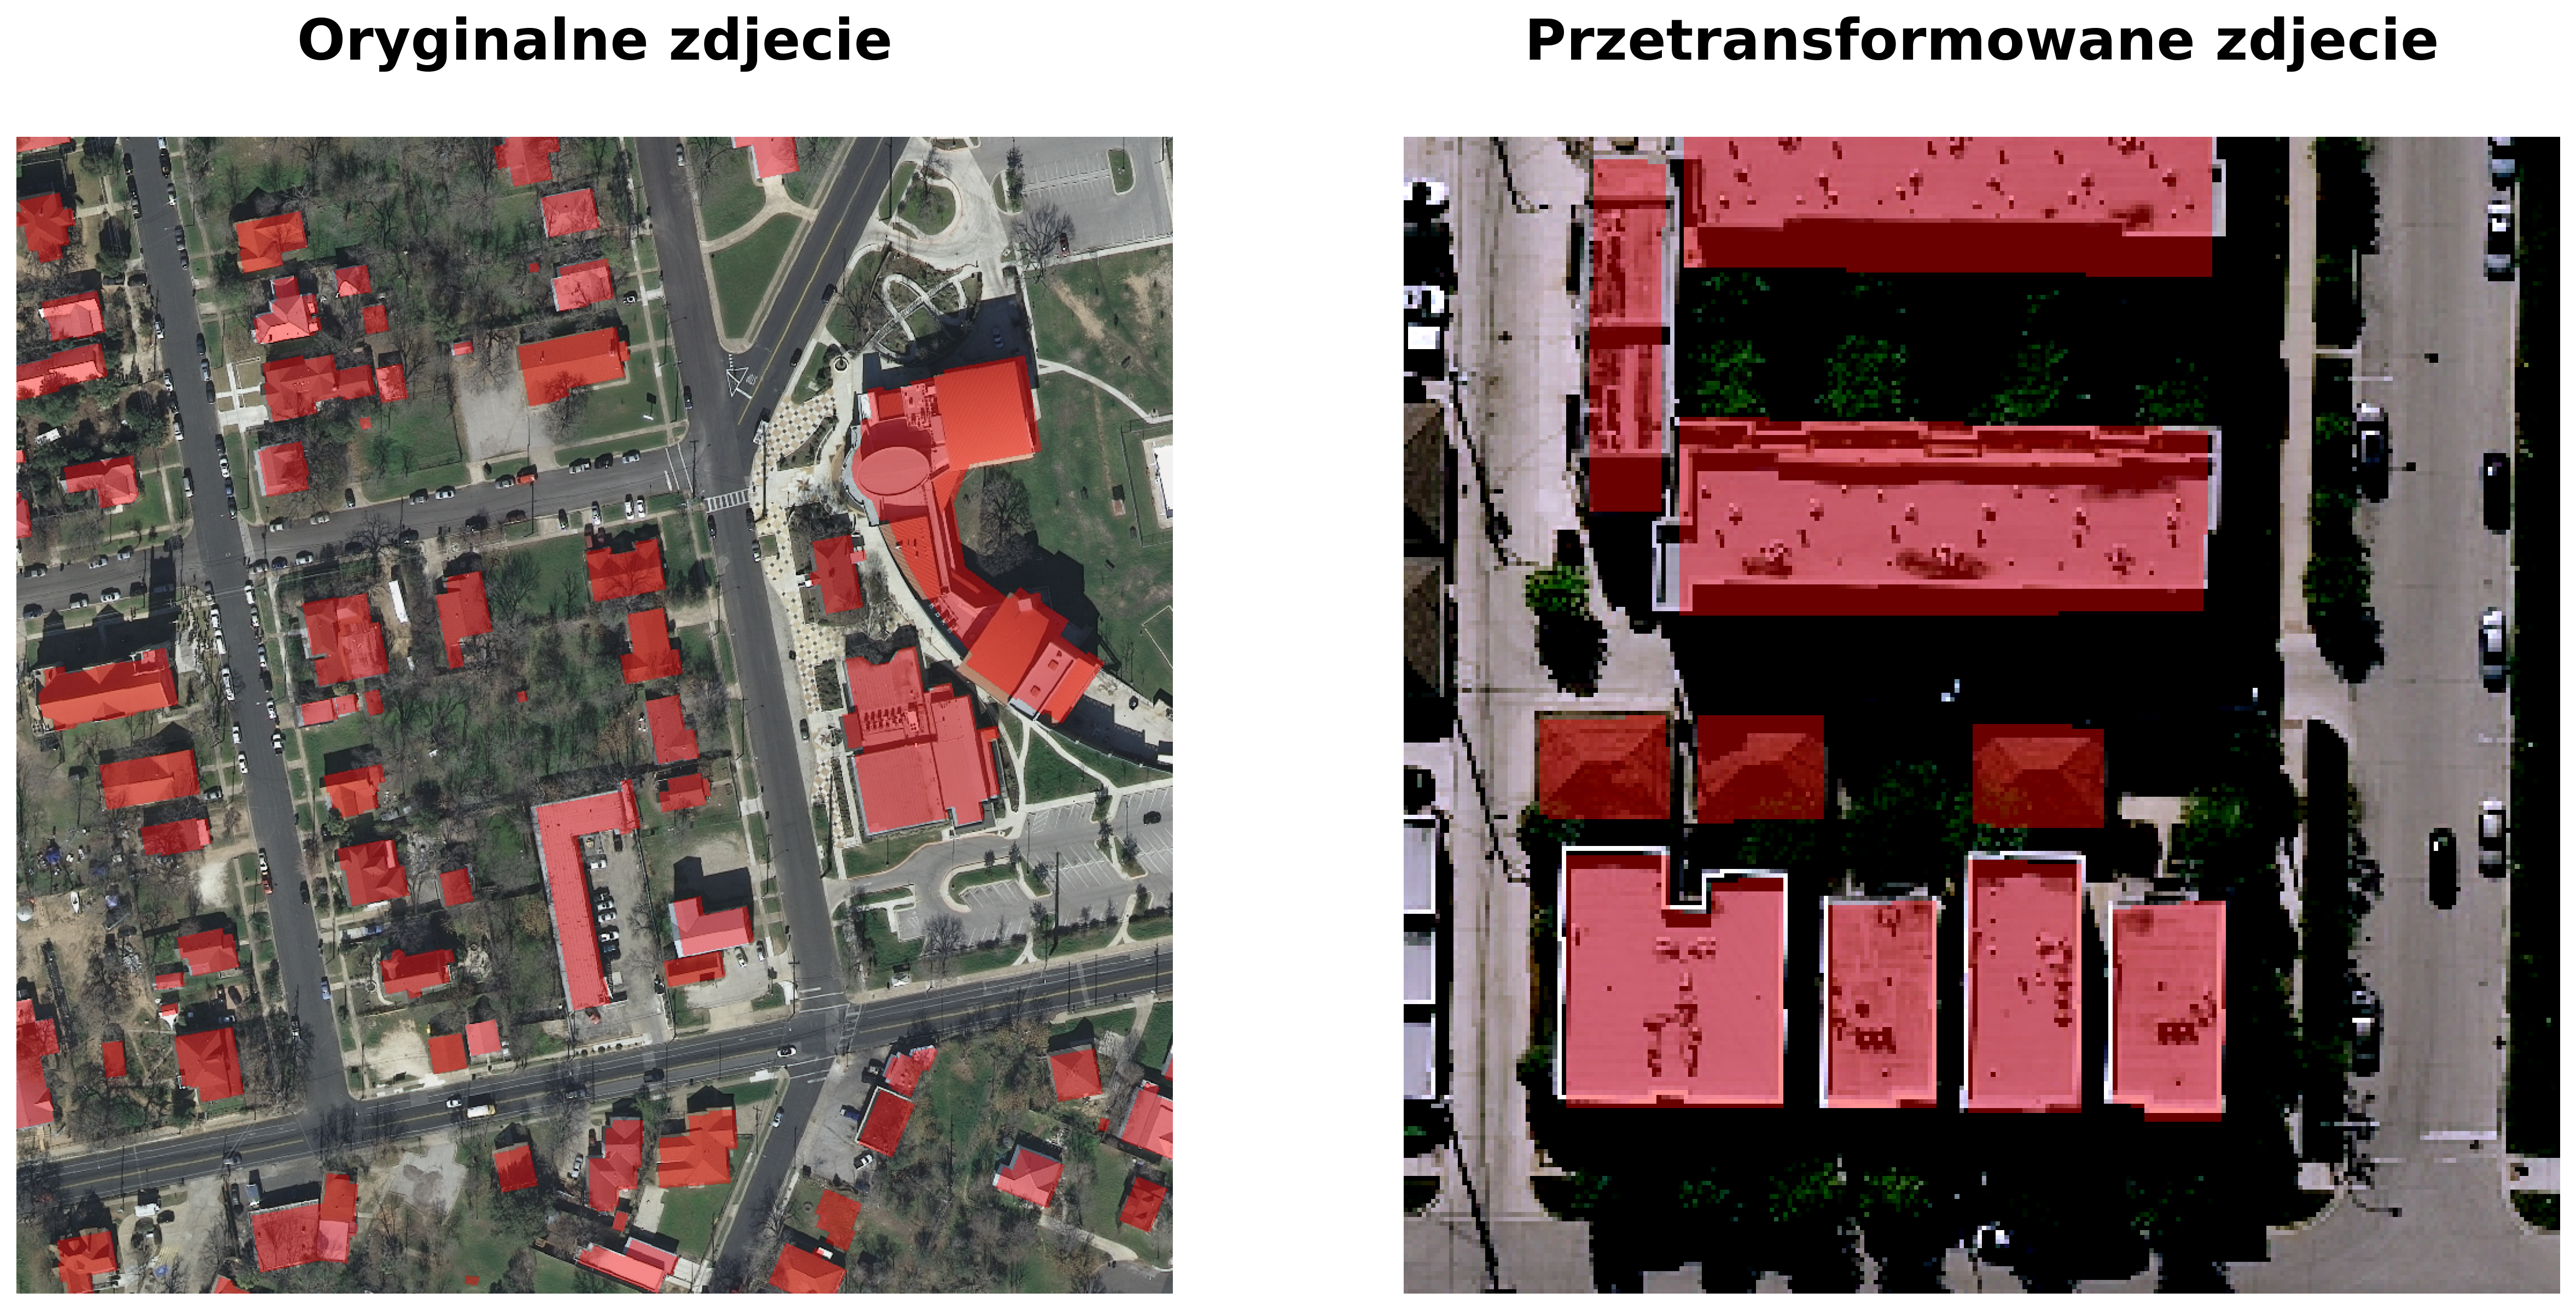
\includegraphics[width=1.0\linewidth]{Org_trans_img.png}
    \captionsetup{format=hang}
    \caption{Porównanie oryginalnego oraz przetransformowanego zdjęcia}
    \label{fig:org_trans1}
\end{figure}

\cell
Ostatnim etapem przygotowywania zbiorów treningowych i walidacyjnych było utworzenie dla nich obiektów ładujących dane (ang. data loader), które posłużyły bezpośrednio do zasilenia finalnego modelu w przykłady uczące / walidacyjne.

\cell
\begin{lstlisting}[name=Rozdzial3.1, language=Python]
train_data_gen = torch.utils.data.DataLoader(train_dataset, shuffle=True, 
                                             batch_size=batch_s, 
                                             num_workers=2, 
                                             pin_memory=True, 
                                             drop_last=True)

valid_data_gen = torch.utils.data.DataLoader(valid_dataset, 
                                             batch_size=batch_s, 
                                             num_workers=2, 
                                             pin_memory=True, 
                                             drop_last=True)

dataset_sizes = {'Train': len(train_data_gen.dataset), 'Valid': 
                 len(valid_data_gen.dataset)}

data_loaders = {'Train': train_data_gen, 'Valid': valid_data_gen}
\end{lstlisting}


\cell
Po ustrukturyzowaniu procesu wczytywania i obróbki danych, kolejnym krokiem  w budowie modelu detekcji budynków na zdjęciach lotniczych, była definicja finalnej architektury sieci $\textit{GML-Net}$.

\vspace{-0.5cm}
\cell
\ss{ Architektura sieci}

\cell
Architektura sieci $\textit{GML-Net}$ wzorowana jest na architekturze $\textit{U-Net}$, jest jednak od niej płytsza o jeden poziom ekstrakcji cech / upsamplingu, stąd też występują w niej tylko trzy połączenia rezydualne. Rolę enkodera w sieci $\textit{GML-Net}$ pełni sieć $\textit{Wide ResNet-50-2}$, która tym różni się od zwykłej sieci $\textit{ResNet-50}$, że posiada dwa razy więcej map cech w blokach rezydualnych, co czyni ją sporo szerszą i w efekcie skuteczniejszą w wychwytywaniu ukrytych zależności. Cechy wyekstraktowane przy pomocy $\textit{Wide ResNet-50-2}$ na danym poziomie rozdzielczości przestrzennej są następnie przetwarzane przez blok $\textit{BottleNeck}$ (wzorowany na blokach sieci $\textit{OSNet}$) po to by uzyskać zagregowany zbiór cech z przekroju różnych skal. Zbiór ten jest następnie transferowany, przy pomocy połączeń rezydualnych, bezpośrednio do warstw dekodera. Rekonstrukcja cech w dekoderze przeprowadzana jest przy pomocy konwolucji transponowanej. Zrekonstruowane cechy są przetwarzane przez blok $\textit{BottleNeck}$, a następnie przeprowadzana jest ich konkatenacja z cechami uzyskanymi z enkodera - tak połączone mapy cech stają się wsadem do kolejnych, wyższych warstw dekodera. W całej sieci powszechnie wykorzystywane są konwolucje separowalne wgłębnie i punktowo, co pozwala sieci $\textit{GML-Net}$ efektywnie nauczyć się korelacji kanałów przestrzennych, uniknąć nadmiernego dopasowania oraz uzyskać większą efektywność obliczeniową. Stąd też pomimo wykorzystania stosunkowo cieżkich architektur jakimi są bez wątpienia $\textit{U-Net}$ i $\textit{Wide ResNet-50-2}$, udało się ograniczyć liczbę trenowalnych parametrów finalnego modelu $\textit{GML-Net}$ do 27 milionów. Rysunek \ref{fig:gmlnet1} przedstawia architekturę omawianej w bieżącym rozdziale sieci:

\begin{figure}[!h]
    \centering \includegraphics[width=1.0\linewidth]{GML-Net.pdf}
    \captionsetup{format=hang}
    \caption{Architektura sieci \textit{GML-Net}}
    \label{fig:gmlnet1}
\end{figure}

Symbole nad poszczególnymi elementami sieci przedstawionej na powyższym rysunku zostały definiowane zgodnie z zapisem $\textit{STNN}$ dla architektur głębokich sieci neuronowych, który został opracowany przez prof. dr. hab. inż. Władysława Skarbka w artykule \textit{Symbolic Tensor Neural Networks for Digital Media – from Tensor Processing via BNF Graph Rules to CREAMS Applications} \cite{skarbek}. Poniżej zaprezentowano szczegółową definicję każdego z tych symboli:

\begin{equation*}
\begin{gathered}
\textbf{Ekstrakcja cech nr 1 - 64 mapy cech, rozdzielczość przestrzenna $\textit{128x128}$ ($\textit{ResNet64}$):}
\\~\\
\xunitdef{\boldsymbol{ResNet}}{\boldsymbol{128:\ 3\rightarrow64}}{\quad
\xinp{256_{xy}}{3}{}{}{}
\xconv{\ 7^k2^s}{\ 64}{p}{}{br}}
\end{gathered}
\end{equation*}
\begin{equation*}
\begin{gathered}
\textbf{Przetworzenie wyekstrahowanych cech $\textit{ResNet64}$ przez blok $\textit{DownBottleNeck64}$:}
\\~\\
\xunitdef{Btlnck64}{1}{\quad
\xunit{ResNet}{128:\ 3\rightarrow64}{} \quad
\xconv{\ 1^k1^s}{\ 16}{}{}{br}}
\\
\xunitdef{Btlnck64}{2}{\quad
\xconv{\ 1^k1^s}{\ 16}{}{}{}
\xconv{\ 3^k1^s}{\ 16}{p}{}{br}}
\\
\xunitdef{Btlnck64}{1-1}{\quad
\xunit{Btlnck64}{1}{} \quad
\xunit{Btlnck64}{2}{}}
\\
\xunitdef{Btlnck64}{1-2}{\quad
\xaggreg{\quad
\xunit{Btlnck64}{1-1}{}
\quad \left|_{\bigotimes} \quad
\xunit{Btlnck64}{1-1}{}
\xpool{g}{}{a}{}{}
\xconv{\ 1^k1^s}{\ 16}{}{}{r}
\xconv{\ 1^k1^s}{\ 16}{}{}{s}
\right.}}
\\
\xunitdef{Btlnck64}{2-1}{\quad
\xunit{Btlnck64}{1-1}{} \quad
\xunit{Btlnck64}{2}{}}
\\
\xunitdef{Btlnck64}{2-2}{\quad
\xaggreg{\quad
\xunit{Btlnck64}{2-1}{}
\quad \left|_{\bigotimes} \quad
\xunit{Btlnck64}{2-1}{}
\xpool{g}{}{a}{}{}
\xconv{\ 1^k1^s}{\ 16}{}{}{r}
\xconv{\ 1^k1^s}{\ 16}{}{}{s}
\right.}}
\\
\xunitdef{Btlnck64}{3-1}{\quad
\xunit{Btlnck64}{2-1}{} \quad
\xunit{Btlnck64}{2}{}}
\\
\xunitdef{Btlnck64}{3-2}{\quad
\xaggreg{\quad
\xunit{Btlnck64}{3-1}{}
\quad \left|_{\bigotimes} \quad
\xunit{Btlnck64}{3-1}{}
\xpool{g}{}{a}{}{}
\xconv{\ 1^k1^s}{\ 16}{}{}{r}
\xconv{\ 1^k1^s}{\ 16}{}{}{s}
\right.}}
\\
\xunitdef{Btlnck64}{4-1}{\quad
\xunit{Btlnck64}{3-1}{} \quad
\xunit{Btlnck64}{2}{}}
\\
\xunitdef{Btlnck64}{4-2}{\quad
\xaggreg{\quad
\xunit{Btlnck64}{4-1}{}
\quad \left|_{\bigotimes} \quad
\xunit{Btlnck64}{4-1}{}
\xpool{g}{}{a}{}{}
\xconv{\ 1^k1^s}{\ 16}{}{}{r}
\xconv{\ 1^k1^s}{\ 16}{}{}{s}
\right.}}
\\
\xunitdef{Btlnck64}{5}{\quad
\xaggreg{\quad
\xaggreg{\quad
\xaggreg{\quad
\xunit{Btlnck64}{1-2}{}
\quad \left|_+ \quad
\xunit{Btlnck64}{2-2}{}
\right.\quad}
\quad \left|_+ \quad
\xunit{Btlnck64}{3-2}{}
\right.\quad}
\quad \left|_+ \quad
\xunit{Btlnck64}{4-2}{}
\right.\quad}}
\\
\xunitdef{\boldsymbol{DownBottleNeck}}{\boldsymbol{128:\ 64\rightarrow64}}{\quad
\xaggreg{\quad
\xunit{ResNet}{128:\ 3\rightarrow64}{}
\quad \left|_+ \quad
\xunit{Btlnck64}{5}{}
\xconv{\ 1^k1^s}{\ 64}{}{}{b}
\right.}^r}
\end{gathered}
\end{equation*}
\begin{equation*}
\begin{gathered}
\textbf{Ekstrakcja cech nr 2 - 256 map cech, rozdzielczość przestrzenna $\textit{64x64}$ ($\textit{ResNet256}$):}
\\~\\
\xunitdef{resnet256}{1}{
\xaggreg{\quad
\xunit{ResNet}{128:\ 3\rightarrow64}{}
\xpool{3^k2^s}{}{mp}{}{}
\xconv{\ 1^k1^s}{\ 128}{}{}{br}
\xconv{\ 3^k1^s}{\ 128}{p}{}{br}
\xconv{\ 1^k1^s}{\ 256}{}{}{b}
\quad \left|_+ \quad
\xunit{ResNet}{128:\ 3\rightarrow64}{}
\xpool{3^k2^s}{}{mp}{}{}
\xconv{\ 1^k1^s}{\ 256}{}{}{b}
\right.}^r}
\\
\xunitdef{resnet256}{2}{
\xaggreg{\quad
\xunit{resnet256}{1}{}
\quad \left|_+ \quad
\xunit{resnet256}{1}{}
\xconv{\ 1^k1^s}{\ 128}{}{}{br}
\xconv{\ 3^k1^s}{\ 128}{p}{}{br}
\xconv{\ 1^k1^s}{\ 256}{}{}{b}
\right.}^r}
\\
\xunitdef{resnet256}{3}{
\xaggreg{\quad
\xunit{resnet256}{2}{}
\quad \left|_+ \quad
\xunit{resnet256}{2}{}
\xconv{\ 1^k1^s}{\ 128}{}{}{br}
\xconv{\ 3^k1^s}{\ 128}{p}{}{br}
\xconv{\ 1^k1^s}{\ 256}{}{}{b}
\right.}^r}
\\
\xunitdef{\boldsymbol{ResNet}}{\boldsymbol{64:\ 64\rightarrow256}}{ \quad
\xunit{resnet256}{1}{} \quad
\xunit{resnet256}{2}{} \quad
\xunit{resnet256}{3}{}}
\end{gathered}
\end{equation*}
\begin{equation*}
\begin{gathered}
\textbf{Przetworzenie wyekstrahowanych cech $\textit{ResNet256}$ przez blok $\textit{DownBottleNeck128}$:}
\\~\\
\xunitdef{Btlnck256}{1}{\quad
\xunit{ResNet}{64\rightarrow256}{} \quad
\xconv{\ 1^k1^s}{\ 32}{}{}{br}}
\\
\xunitdef{Btlnck256}{2}{\quad
\xconv{\ 1^k1^s}{\ 32}{}{}{}
\xconv{\ 3^k1^s}{\ 32}{p}{}{br}}
\\
\xunitdef{Btlnck256}{1-1}{\quad
\xunit{Btlnck256}{1}{} \quad
\xunit{Btlnck256}{2}{}}
\\
\xunitdef{Btlnck256}{1-2}{\quad
\xaggreg{\quad
\xunit{Btlnck256}{1-1}{}
\quad \left|_{\bigotimes} \quad
\xunit{Btlnck256}{1-1}{}
\xpool{g}{}{a}{}{}
\xconv{\ 1^k1^s}{\ 32}{}{}{r}
\xconv{\ 1^k1^s}{\ 32}{}{}{s}
\right.}}
\\
\xunitdef{Btlnck256}{2-1}{\quad
\xunit{Btlnck256}{1-1}{} \quad
\xunit{Btlnck256}{2}{}}
\\
\xunitdef{Btlnck256}{2-2}{\quad
\xaggreg{\quad
\xunit{Btlnck256}{2-1}{}
\quad \left|_{\bigotimes} \quad
\xunit{Btlnck256}{2-1}{}
\xpool{g}{}{a}{}{}
\xconv{\ 1^k1^s}{\ 32}{}{}{r}
\xconv{\ 1^k1^s}{\ 32}{}{}{s}
\right.}}
\\
\xunitdef{Btlnck256}{3-1}{\quad
\xunit{Btlnck256}{2-1}{} \quad
\xunit{Btlnck256}{2}{}}
\\
\xunitdef{Btlnck256}{3-2}{\quad
\xaggreg{\quad
\xunit{Btlnck256}{3-1}{}
\quad \left|_{\bigotimes} \quad
\xunit{Btlnck256}{3-1}{}
\xpool{g}{}{a}{}{}
\xconv{\ 1^k1^s}{\ 32}{}{}{r}
\xconv{\ 1^k1^s}{\ 32}{}{}{s}
\right.}}
\end{gathered}
\end{equation*}
\begin{equation*}
\begin{gathered}
\xunitdef{Btlnck256}{4-1}{\quad
\xunit{Btlnck256}{3-1}{} \quad
\xunit{Btlnck256}{2}{}}
\\
\xunitdef{Btlnck256}{4-2}{\quad
\xaggreg{\quad
\xunit{Btlnck256}{4-1}{}
\quad \left|_{\bigotimes} \quad
\xunit{Btlnck256}{4-1}{}
\xpool{g}{}{a}{}{}
\xconv{\ 1^k1^s}{\ 32}{}{}{r}
\xconv{\ 1^k1^s}{\ 32}{}{}{s}
\right.}}
\\
\xunitdef{Btlnck256}{5}{\quad
\xaggreg{\quad
\xaggreg{\quad
\xaggreg{\quad
\xunit{Btlnck256}{1-2}{}
\quad \left|_+ \quad
\xunit{Btlnck256}{2-2}{}
\right.\quad}
\quad \left|_+ \quad
\xunit{Btlnck256}{3-2}{}
\right.\quad}
\quad \left|_+ \quad
\xunit{Btlnck256}{4-2}{}
\right.\quad}}
\\
\xunitdef{\boldsymbol{DownBottleNeck}}{\boldsymbol{64:\ 256\rightarrow128}}{\quad
\xaggreg{\quad
\xunit{ResNet}{64\rightarrow256}{}
\xconv{\ 1^k1^s}{\ 128}{}{}{b}
\quad \left|_+ \quad
\xunit{Btlnck256}{5}{}
\xconv{\ 1^k1^s}{\ 128}{}{}{b}
\right.}^r}
\end{gathered}
\end{equation*}
\begin{equation*}
\begin{gathered}
\textbf{Ekstrakcja cech nr 3 - 512 map cech, rozdzielczość przestrzenna $\textit{32x32}$ ($\textit{ResNet512}$):}
\\~\\
\xunitdef{resnet512}{1}{
\xaggreg{\quad
\xunit{ResNet}{64\rightarrow256}{}
\xconv{\ 1^k1^s}{\ 256}{}{}{br}
\xconv{\ 3^k2^s}{\ 256}{p}{}{br}
\xconv{\ 1^k1^s}{\ 512}{}{}{b}
\quad \left|_+ \quad
\xunit{ResNet}{64\rightarrow256}{}
\xconv{\ 1^k2^s}{\ 512}{}{}{b}
\right.}^r}
\\
\xunitdef{resnet512}{2}{
\xaggreg{\quad
\xunit{resnet512}{1}{}
\quad \left|_+ \quad
\xunit{resnet512}{1}{}
\xconv{\ 1^k1^s}{\ 256}{}{}{br}
\xconv{\ 3^k1^s}{\ 256}{p}{}{br}
\xconv{\ 1^k1^s}{\ 512}{}{}{b}
\right.}^r}
\\
\xunitdef{resnet512}{3}{
\xaggreg{\quad
\xunit{resnet512}{2}{}
\quad \left|_+ \quad
\xunit{resnet512}{2}{}
\xconv{\ 1^k1^s}{\ 256}{}{}{br}
\xconv{\ 3^k1^s}{\ 256}{p}{}{br}
\xconv{\ 1^k1^s}{\ 512}{}{}{b}
\right.}^r}
\\
\xunitdef{resnet512}{4}{
\xaggreg{\quad
\xunit{resnet512}{3}{}
\quad \left|_+ \quad
\xunit{resnet512}{3}{}
\xconv{\ 1^k1^s}{\ 256}{}{}{br}
\xconv{\ 3^k1^s}{\ 256}{p}{}{br}
\xconv{\ 1^k1^s}{\ 512}{}{}{b}
\right.}^r}
\\
\xunitdef{\boldsymbol{ResNet}}{\boldsymbol{32:\ 256\rightarrow512}}{ \quad
\xunit{resnet512}{1}{} \quad
\xunit{resnet512}{2}{} \quad
\xunit{resnet512}{3}{} \quad
\xunit{resnet512}{4}{}}
\end{gathered}
\end{equation*}
\begin{equation*}
\begin{gathered}
\textbf{Przetworzenie wyekstrahowanych cech $\textit{ResNet512}$ przez blok $\textit{DownBottleNeck256}$:}
\\~\\
\xunitdef{Btlnck512}{1}{\quad
\xunit{ResNet}{32:\ 256\rightarrow512}{} \quad
\xconv{\ 1^k1^s}{\ 64}{}{}{br}}
\\
\xunitdef{Btlnck512}{2}{\quad
\xconv{\ 1^k1^s}{\ 64}{}{}{}
\xconv{\ 3^k1^s}{\ 64}{p}{}{br}}
\\
\xunitdef{Btlnck512}{1-1}{\quad
\xunit{Btlnck512}{1}{} \quad
\xunit{Btlnck512}{2}{}}
\end{gathered}
\end{equation*}
\begin{equation*}
\begin{gathered}
\xunitdef{Btlnck512}{1-2}{\quad
\xaggreg{\quad
\xunit{Btlnck512}{1-1}{}
\quad \left|_{\bigotimes} \quad
\xunit{Btlnck512}{1-1}{}
\xpool{g}{}{a}{}{}
\xconv{\ 1^k1^s}{\ 64}{}{}{r}
\xconv{\ 1^k1^s}{\ 64}{}{}{s}
\right.}}
\\
\xunitdef{Btlnck512}{2-1}{\quad
\xunit{Btlnck512}{1-1}{} \quad
\xunit{Btlnck512}{2}{}}
\\
\xunitdef{Btlnck512}{2-2}{\quad
\xaggreg{\quad
\xunit{Btlnck512}{2-1}{}
\quad \left|_{\bigotimes} \quad
\xunit{Btlnck512}{2-1}{}
\xpool{g}{}{a}{}{}
\xconv{\ 1^k1^s}{\ 64}{}{}{r}
\xconv{\ 1^k1^s}{\ 64}{}{}{s}
\right.}}
\\
\xunitdef{Btlnck512}{3-1}{\quad
\xunit{Btlnck512}{2-1}{} \quad
\xunit{Btlnck512}{2}{}}
\\
\xunitdef{Btlnck512}{3-2}{\quad
\xaggreg{\quad
\xunit{Btlnck512}{3-1}{}
\quad \left|_{\bigotimes} \quad
\xunit{Btlnck512}{3-1}{}
\xpool{g}{}{a}{}{}
\xconv{\ 1^k1^s}{\ 64}{}{}{r}
\xconv{\ 1^k1^s}{\ 64}{}{}{s}
\right.}}
\\
\xunitdef{Btlnck512}{4-1}{\quad
\xunit{Btlnck512}{3-1}{} \quad
\xunit{Btlnck512}{2}{}}
\\
\xunitdef{Btlnck512}{4-2}{\quad
\xaggreg{\quad
\xunit{Btlnck512}{4-1}{}
\quad \left|_{\bigotimes} \quad
\xunit{Btlnck512}{4-1}{}
\xpool{g}{}{a}{}{}
\xconv{\ 1^k1^s}{\ 64}{}{}{r}
\xconv{\ 1^k1^s}{\ 64}{}{}{s}
\right.}}
\\
\xunitdef{Btlnck512}{5}{\quad
\xaggreg{\quad
\xaggreg{\quad
\xaggreg{\quad
\xunit{Btlnck512}{1-2}{}
\quad \left|_+ \quad
\xunit{Btlnck512}{2-2}{}
\right.\quad}
\quad \left|_+ \quad
\xunit{Btlnck512}{3-2}{}
\right.\quad}
\quad \left|_+ \quad
\xunit{Btlnck512}{4-2}{}
\right.\quad}}
\\
\xunitdef{\boldsymbol{DownBottleNeck}}{\boldsymbol{32:\ 512\rightarrow256}}{\quad
\xaggreg{\quad
\xunit{ResNet}{32:\ 256\rightarrow512}{}
\xconv{\ 1^k1^s}{\ 256}{}{}{b}
\quad \left|_+ \quad
\xunit{Btlnck512}{5}{}
\xconv{\ 1^k1^s}{\ 256}{}{}{b}
\right.}^r}
\end{gathered}
\end{equation*}
\begin{equation*}
\begin{gathered}
\textbf{Ekstrakcja cech nr 4 - 1024 mapy cech, rozdzielczość przestrzenna $\textit{16x16}$ ($\textit{ResNet1024}$):}
\\~\\
\xunitdef{resnet1024}{1}{
\xaggreg{\quad
\xunit{ResNet}{32:\ 256-512}{}
\xconv{\ 1^k1^s}{\ 512}{}{}{br}
\xconv{\ 3^k2^s}{\ 512}{p}{}{br}
\xconv{\ 1^k1^s}{\ 1024}{}{}{b}
\quad \left|_+ \quad
\xunit{ResNet}{32:\ 256-512}{}
\xconv{\ 1^k2^s}{\ 1024}{}{}{b}
\right.}^r}
\\
\xunitdef{resnet1024}{2}{
\xaggreg{\quad
\xunit{resnet1024}{1}{}
\quad \left|_+ \quad
\xunit{resnet1024}{1}{}
\xconv{\ 1^k1^s}{\ 512}{}{}{br}
\xconv{\ 3^k1^s}{\ 512}{p}{}{br}
\xconv{\ 1^k1^s}{\ 1024}{}{}{b}
\right.}^r}
\\
\xunitdef{resnet1024}{3}{
\xaggreg{\quad
\xunit{resnet1024}{2}{}
\quad \left|_+ \quad
\xunit{resnet1024}{2}{}
\xconv{\ 1^k1^s}{\ 512}{}{}{br}
\xconv{\ 3^k1^s}{\ 512}{p}{}{br}
\xconv{\ 1^k1^s}{\ 1024}{}{}{b}
\right.}^r}
\\
\xunitdef{resnet1024}{4}{
\xaggreg{\quad
\xunit{resnet1024}{3}{}
\quad \left|_+ \quad
\xunit{resnet1024}{3}{}
\xconv{\ 1^k1^s}{\ 512}{}{}{br}
\xconv{\ 3^k1^s}{\ 512}{p}{}{br}
\xconv{\ 1^k1^s}{\ 1024}{}{}{b}
\right.}^r}
\end{gathered}
\end{equation*}
\begin{equation*}
\begin{gathered}
\xunitdef{resnet1024}{5}{
\xaggreg{\quad
\xunit{resnet1024}{4}{}
\quad \left|_+ \quad
\xunit{resnet1024}{4}{}
\xconv{\ 1^k1^s}{\ 512}{}{}{br}
\xconv{\ 3^k1^s}{\ 512}{p}{}{br}
\xconv{\ 1^k1^s}{\ 1024}{}{}{b}
\right.}^r}
\\
\xunitdef{resnet1024}{6}{
\xaggreg{\quad
\xunit{resnet1024}{5}{}
\quad \left|_+ \quad
\xunit{resnet1024}{5}{}
\xconv{\ 1^k1^s}{\ 512}{}{}{br}
\xconv{\ 3^k1^s}{\ 512}{p}{}{br}
\xconv{\ 1^k1^s}{\ 1024}{}{}{b}
\right.}^r}
\\
\xunitdef{\boldsymbol{ResNet}}{\boldsymbol{16:\ 512-1024}}{ \quad
\xunit{resnet1024}{1}{} \quad
\xunit{resnet1024}{2}{} \quad
\xunit{resnet1024}{3}{} \quad
\xunit{resnet1024}{4}{} \quad
\xunit{resnet1024}{5}{}\quad
\xunit{resnet1024}{6}{}}
\end{gathered}
\end{equation*}
\begin{equation*}
\begin{gathered}
\textbf{Przetworzenie wyekstrahowanych cech $\textit{ResNet1024}$ przez blok $\textit{DownBottleNeck512}$:}
\\~\\
\xunitdef{Btlnck1024}{1}{\quad
\xunit{ResNet}{16:\ 512\rightarrow1024}{} \quad
\xconv{\ 1^k1^s}{\ 128}{}{}{br}}
\\
\xunitdef{Btlnck1024}{2}{\quad
\xconv{\ 1^k1^s}{\ 128}{}{}{}
\xconv{\ 3^k1^s}{\ 128}{p}{}{br}}
\\
\xunitdef{Btlnck1024}{1-1}{\quad
\xunit{Btlnck1024}{1}{} \quad
\xunit{Btlnck1024}{2}{}}
\\
\xunitdef{Btlnck1024}{1-2}{\quad
\xaggreg{\quad
\xunit{Btlnck1024}{1-1}{}
\quad \left|_{\bigotimes} \quad
\xunit{Btlnck1024}{1-1}{}
\xpool{g}{}{a}{}{}
\xconv{\ 1^k1^s}{\ 128}{}{}{r}
\xconv{\ 1^k1^s}{\ 128}{}{}{s}
\right.}}
\\
\xunitdef{Btlnck1024}{2-1}{\quad
\xunit{Btlnck1024}{1-1}{} \quad
\xunit{Btlnck1024}{2}{}}
\\
\xunitdef{Btlnck1024}{2-2}{\quad
\xaggreg{\quad
\xunit{Btlnck1024}{2-1}{}
\quad \left|_{\bigotimes} \quad
\xunit{Btlnck1024}{2-1}{}
\xpool{g}{}{a}{}{}
\xconv{\ 1^k1^s}{\ 128}{}{}{r}
\xconv{\ 1^k1^s}{\ 128}{}{}{s}
\right.}}
\\
\xunitdef{Btlnck1024}{3-1}{\quad
\xunit{Btlnck1024}{2-1}{} \quad
\xunit{Btlnck1024}{2}{}}
\\
\xunitdef{Btlnck1024}{3-2}{\quad
\xaggreg{\quad
\xunit{Btlnck1024}{3-1}{}
\quad \left|_{\bigotimes} \quad
\xunit{Btlnck1024}{3-1}{}
\xpool{g}{}{a}{}{}
\xconv{\ 1^k1^s}{\ 128}{}{}{r}
\xconv{\ 1^k1^s}{\ 128}{}{}{s}
\right.}}
\\
\xunitdef{Btlnck1024}{4-1}{\quad
\xunit{Btlnck1024}{3-1}{} \quad
\xunit{Btlnck1024}{2}{}}
\\
\xunitdef{Btlnck1024}{4-2}{\quad
\xaggreg{\quad
\xunit{Btlnck1024}{4-1}{}
\quad \left|_{\bigotimes} \quad
\xunit{Btlnck1024}{4-1}{}
\xpool{g}{}{a}{}{}
\xconv{\ 1^k1^s}{\ 128}{}{}{r}
\xconv{\ 1^k1^s}{\ 128}{}{}{s}
\right.}}
\\
\xunitdef{Btlnck1024}{5}{\quad
\xaggreg{\quad
\xaggreg{\quad
\xaggreg{\quad
\xunit{Btlnck1024}{1-2}{}
\quad \left|_+ \quad
\xunit{Btlnck1024}{2-2}{}
\right.\quad}
\quad \left|_+ \quad
\xunit{Btlnck1024}{3-2}{}
\right.\quad}
\quad \left|_+ \quad
\xunit{Btlnck1024}{4-2}{}
\right.\quad}}
\end{gathered}
\end{equation*}
\begin{equation*}
\begin{gathered}
\xunitdef{\boldsymbol{DownBottleNeck}}{\boldsymbol{16:\ 1024\rightarrow512}}{\quad
\xaggreg{\quad
\xunit{ResNet}{16:\ 512\rightarrow1024}{}
\xconv{\ 1^k1^s}{\ 512}{}{}{b}
\quad \left|_+ \quad
\xunit{Btlnck1024}{5}{}
\xconv{\ 1^k1^s}{\ 512}{}{}{b}
\right.}^r}
\end{gathered}
\end{equation*}
\begin{equation*}
\begin{gathered}
\textbf{Rekonstrukcja nr 1 - 256 map cech, rozdzielczość przestrzenna $\textit{32x32}$ ($\textit{TransConv256}$):}
\\~\\
\xunitdef{\boldsymbol{TransConv}}{\boldsymbol{32:\ 512\rightarrow256}}{\quad
\xunit{DownBottleNeck}{16:\ 1024\rightarrow512}{}
\xconv{\ 1^k1^s}{\ 256}{}{}{}
\xconv{\ 1^k1^s}{\ 256}{}{}{r}
\xconv{\ 2^k2^s}{\ 256}{t}{}{}}
\end{gathered}
\end{equation*}
\begin{equation*}
\begin{gathered}
\textbf{Przetworzenie nadpróbkowanych cech $\textit{TransConv256}$ przez blok $\textit{UpBottleNeck192}$:}
\\~\\
\xunitdef{UpBtnk256}{1}{\quad
\xunit{TransConv}{32:\ 512\rightarrow256}{} \quad
\xconv{\ 1^k1^s}{\ 48}{}{}{br}}
\\
\xunitdef{UpBtnk256}{2}{\quad
\xconv{\ 1^k1^s}{\ 48}{}{}{}
\xconv{\ 3^k1^s}{\ 48}{p}{}{br}}
\\
\xunitdef{UpBtnk256}{1-1}{\quad
\xunit{UpBtnk256}{1}{} \quad
\xunit{UpBtnk256}{2}{}}
\\
\xunitdef{UpBtnk256}{1-2}{\quad
\xaggreg{\quad
\xunit{UpBtnk256}{1-1}{}
\quad \left|_{\bigotimes} \quad
\xunit{UpBtnk256}{1-1}{}
\xpool{g}{}{a}{}{}
\xconv{\ 1^k1^s}{\ 48}{}{}{r}
\xconv{\ 1^k1^s}{\ 48}{}{}{s}
\right.}}
\\
\xunitdef{UpBtnk256}{2-1}{\quad
\xunit{UpBtnk256}{1-1}{} \quad
\xunit{UpBtnk256}{2}{}}
\\
\xunitdef{UpBtnk256}{2-2}{\quad
\xaggreg{\quad
\xunit{UpBtnk256}{2-1}{}
\quad \left|_{\bigotimes} \quad
\xunit{UpBtnk256}{2-1}{}
\xpool{g}{}{a}{}{}
\xconv{\ 1^k1^s}{\ 48}{}{}{r}
\xconv{\ 1^k1^s}{\ 48}{}{}{s}
\right.}}
\\
\xunitdef{UpBtnk256}{3-1}{\quad
\xunit{UpBtnk256}{2-1}{} \quad
\xunit{UpBtnk256}{2}{}}
\\
\xunitdef{UpBtnk256}{3-2}{\quad
\xaggreg{\quad
\xunit{UpBtnk256}{3-1}{}
\quad \left|_{\bigotimes} \quad
\xunit{UpBtnk256}{3-1}{}
\xpool{g}{}{a}{}{}
\xconv{\ 1^k1^s}{\ 48}{}{}{r}
\xconv{\ 1^k1^s}{\ 48}{}{}{s}
\right.}}
\\
\xunitdef{UpBtnk256}{4-1}{\quad
\xunit{UpBtnk256}{3-1}{} \quad
\xunit{UpBtnk256}{2}{}}
\\
\xunitdef{UpBtnk256}{4-2}{\quad
\xaggreg{\quad
\xunit{UpBtnk256}{4-1}{}
\quad \left|_{\bigotimes} \quad
\xunit{UpBtnk256}{4-1}{}
\xpool{g}{}{a}{}{}
\xconv{\ 1^k1^s}{\ 48}{}{}{r}
\xconv{\ 1^k1^s}{\ 48}{}{}{s}
\right.}}
\end{gathered}
\end{equation*}
\begin{equation*}
\begin{gathered}
\xunitdef{UpBtnk256}{5}{\quad
\xaggreg{\quad
\xaggreg{\quad
\xaggreg{\quad
\xunit{UpBtnk256}{1-2}{}
\quad \left|_+ \quad
\xunit{UpBtnk256}{2-2}{}
\right.\quad}
\quad \left|_+ \quad
\xunit{UpBtnk256}{3-2}{}
\right.\quad}
\quad \left|_+ \quad
\xunit{UpBtnk256}{4-2}{}
\right.\quad}}
\\
\xunitdef{\boldsymbol{UpBottleNeck}}{\boldsymbol{32:\ 256\rightarrow192}}{\quad
\xaggreg{\quad
\xunit{TransConv}{32:\ 512\rightarrow256}{}
\xconv{\ 1^k1^s}{\ 192}{}{}{b}
\quad \left|_+ \quad
\xunit{UpBtnk256}{5}{}
\xconv{\ 1^k1^s}{\ 192}{}{}{b}
\right.}^r}
\end{gathered}
\end{equation*}
\begin{equation*}
\begin{gathered}
\textbf{Konkatenacja nr 1 - 448 map cech, rozdzielczość przestrzenna $\textit{32x32}$ ($\textit{ConCat448}$):}
\\~\\
\xunitdef{\boldsymbol{ConCat}}{\boldsymbol{32:\ \langle \; 256 \; | \; 192 \; \rangle}}{\quad
\xaggreg{\quad
\xunit{UpBottleNeck}{32:\ 256\rightarrow192}{}
\quad \left| \quad
\xunit{DownBottleNeck}{32:\ 512\rightarrow256}{}
\right.}}
\end{gathered}
\end{equation*}
\begin{equation*}
\begin{gathered}
\textbf{Rekonstrukcja nr 2 - 192 mapy cech, rozdzielczość przestrzenna $\textit{64x64}$ ($\textit{TransConv192}$):}
\\~\\
\xunitdef{\boldsymbol{TransConv}}{\boldsymbol{64:\ 448\rightarrow192}}{\quad
\xunit{ConCat}{32:\ \langle \; 256 \; | \; 192 \; \rangle}{}
\xconv{\ 1^k1^s}{\ 192}{}{}{}
\xconv{\ 3^k1^s}{\ 192}{p}{}{br}
\xconv{\ 2^k2^s}{\ 192}{t}{}{}}
\end{gathered}
\end{equation*}
\begin{equation*}
\begin{gathered}
\textbf{Przetworzenie nadpróbkowanych cech $\textit{TransConv192}$ przez blok $\textit{UpBottleNeck128}$:}
\\~\\
\xunitdef{UpBtnk128}{1}{\quad
\xunit{TransConv}{64:\ 448\rightarrow192}{} \quad
\xconv{\ 1^k1^s}{\ 32}{}{}{br}}
\\
\xunitdef{UpBtnk128}{2}{\quad
\xconv{\ 1^k1^s}{\ 32}{}{}{}
\xconv{\ 3^k1^s}{\ 32}{p}{}{br}}
\\
\xunitdef{UpBtnk128}{1-1}{\quad
\xunit{UpBtnk128}{1}{} \quad
\xunit{UpBtnk128}{2}{}}
\\
\xunitdef{UpBtnk128}{1-2}{\quad
\xaggreg{\quad
\xunit{UpBtnk128}{1-1}{}
\quad \left|_{\bigotimes} \quad
\xunit{UpBtnk128}{1-1}{}
\xpool{g}{}{a}{}{}
\xconv{\ 1^k1^s}{\ 32}{}{}{r}
\xconv{\ 1^k1^s}{\ 32}{}{}{s}
\right.}}
\\
\xunitdef{UpBtnk128}{2-1}{\quad
\xunit{UpBtnk128}{1-1}{} \quad
\xunit{UpBtnk128}{2}{}}
\\
\xunitdef{UpBtnk128}{2-2}{\quad
\xaggreg{\quad
\xunit{UpBtnk128}{2-1}{}
\quad \left|_{\bigotimes} \quad
\xunit{UpBtnk128}{2-1}{}
\xpool{g}{}{a}{}{}
\xconv{\ 1^k1^s}{\ 32}{}{}{r}
\xconv{\ 1^k1^s}{\ 32}{}{}{s}
\right.}}
\end{gathered}
\end{equation*}
\begin{equation*}
\begin{gathered}
\xunitdef{UpBtnk128}{3-1}{\quad
\xunit{UpBtnk128}{2-1}{} \quad
\xunit{UpBtnk128}{2}{}}
\\
\xunitdef{UpBtnk128}{3-2}{\quad
\xaggreg{\quad
\xunit{UpBtnk128}{3-1}{}
\quad \left|_{\bigotimes} \quad
\xunit{UpBtnk128}{3-1}{}
\xpool{g}{}{a}{}{}
\xconv{\ 1^k1^s}{\ 32}{}{}{r}
\xconv{\ 1^k1^s}{\ 32}{}{}{s}
\right.}}
\\
\xunitdef{UpBtnk128}{4-1}{\quad
\xunit{UpBtnk128}{3-1}{} \quad
\xunit{UpBtnk128}{2}{}}
\\
\xunitdef{UpBtnk128}{4-2}{\quad
\xaggreg{\quad
\xunit{UpBtnk128}{4-1}{}
\quad \left|_{\bigotimes} \quad
\xunit{UpBtnk128}{4-1}{}
\xpool{g}{}{a}{}{}
\xconv{\ 1^k1^s}{\ 32}{}{}{r}
\xconv{\ 1^k1^s}{\ 32}{}{}{s}
\right.}}
\\
\xunitdef{UpBtnk128}{5}{\quad
\xaggreg{\quad
\xaggreg{\quad
\xaggreg{\quad
\xunit{UpBtnk128}{1-2}{}
\quad \left|_+ \quad
\xunit{UpBtnk128}{2-2}{}
\right.\quad}
\quad \left|_+ \quad
\xunit{UpBtnk128}{3-2}{}
\right.\quad}
\quad \left|_+ \quad
\xunit{UpBtnk128}{4-2}{}
\right.\quad}}
\\
\xunitdef{\boldsymbol{UpBottleNeck}}{\boldsymbol{64:\ 192\rightarrow128}}{\quad
\xaggreg{\quad
\xunit{TransConv}{64:\ 448\rightarrow192}{}
\xconv{\ 1^k1^s}{\ 128}{}{}{b}
\quad \left|_+ \quad
\xunit{UpBtnk128}{5}{}
\xconv{\ 1^k1^s}{\ 128}{}{}{b}
\right.}^r}
\end{gathered}
\end{equation*}
\begin{equation*}
\begin{gathered}
\textbf{Konkatenacja nr 2 - 256 map cech, rozdzielczość przestrzenna $\textit{64x64}$ ($\textit{ConCat256}$):}
\\~\\
\xunitdef{\boldsymbol{ConCat}}{\boldsymbol{64:\ \langle \; 128 \; | \; 128 \; \rangle}}{\quad
\xaggreg{\quad
\xunit{UpBottleNeck}{64:\ 192\rightarrow128}{}
\quad \left| \quad
\xunit{DownBottleNeck}{64:\ 256\rightarrow128}{}
\right.}}
\end{gathered}
\end{equation*}
\begin{equation*}
\begin{gathered}
\textbf{Rekonstrukcja nr 3 - 128 map cech, rozdzielczość przestrzenna $\textit{128x128}$ ($\textit{TransConv128}$):}
\\~\\
\xunitdef{\boldsymbol{TransConv}}{\boldsymbol{128:\ 256\rightarrow128}}{\quad
\xunit{ConCat}{64:\ \langle \; 128 \; | \; 128 \; \rangle}{}
\xconv{\ 1^k1^s}{\ 128}{}{}{}
\xconv{\ 3^k1^s}{\ 128}{p}{}{br}
\xconv{\ 2^k2^s}{\ 128}{t}{}{}}
\end{gathered}
\end{equation*}
\begin{equation*}
\begin{gathered}
\textbf{Przetworzenie nadpróbkowanych cech $\textit{TransConv128}$ przez blok $\textit{UpBottleNeck64}$:}
\\~\\
\xunitdef{UpBtnk64}{1}{\quad
\xunit{TransConv}{128:\ 256\rightarrow128}{} \quad
\xconv{\ 1^k1^s}{\ 16}{}{}{br}}
\\
\xunitdef{UpBtnk64}{2}{\quad
\xconv{\ 1^k1^s}{\ 16}{}{}{}
\xconv{\ 3^k1^s}{\ 16}{p}{}{br}}
\end{gathered}
\end{equation*}
\begin{equation*}
\begin{gathered}
\xunitdef{UpBtnk64}{1-1}{\quad
\xunit{UpBtnk64}{1}{} \quad
\xunit{UpBtnk64}{2}{}}
\\
\xunitdef{UpBtnk64}{1-2}{\quad
\xaggreg{\quad
\xunit{UpBtnk64}{1-1}{}
\quad \left|_{\bigotimes} \quad
\xunit{UpBtnk64}{1-1}{}
\xpool{g}{}{a}{}{}
\xconv{\ 1^k1^s}{\ 16}{}{}{r}
\xconv{\ 1^k1^s}{\ 16}{}{}{s}
\right.}}
\\
\xunitdef{UpBtnk64}{2-1}{\quad
\xunit{UpBtnk64}{1-1}{} \quad
\xunit{UpBtnk64}{2}{}}
\\
\xunitdef{UpBtnk64}{2-2}{\quad
\xaggreg{\quad
\xunit{UpBtnk64}{2-1}{}
\quad \left|_{\bigotimes} \quad
\xunit{UpBtnk64}{2-1}{}
\xpool{g}{}{a}{}{}
\xconv{\ 1^k1^s}{\ 16}{}{}{r}
\xconv{\ 1^k1^s}{\ 16}{}{}{s}
\right.}}
\\
\xunitdef{UpBtnk64}{3-1}{\quad
\xunit{UpBtnk64}{2-1}{} \quad
\xunit{UpBtnk64}{2}{}}
\\
\xunitdef{UpBtnk64}{3-2}{\quad
\xaggreg{\quad
\xunit{UpBtnk64}{3-1}{}
\quad \left|_{\bigotimes} \quad
\xunit{UpBtnk64}{3-1}{}
\xpool{g}{}{a}{}{}
\xconv{\ 1^k1^s}{\ 16}{}{}{r}
\xconv{\ 1^k1^s}{\ 16}{}{}{s}
\right.}}
\\
\xunitdef{UpBtnk64}{4-1}{\quad
\xunit{UpBtnk64}{3-1}{} \quad
\xunit{UpBtnk64}{2}{}}
\\
\xunitdef{UpBtnk64}{4-2}{\quad
\xaggreg{\quad
\xunit{UpBtnk64}{4-1}{}
\quad \left|_{\bigotimes} \quad
\xunit{UpBtnk64}{4-1}{}
\xpool{g}{}{a}{}{}
\xconv{\ 1^k1^s}{\ 16}{}{}{r}
\xconv{\ 1^k1^s}{\ 16}{}{}{s}
\right.}}
\\
\xunitdef{UpBtnk64}{5}{\quad
\xaggreg{\quad
\xaggreg{\quad
\xaggreg{\quad
\xunit{UpBtnk64}{1-2}{}
\quad \left|_+ \quad
\xunit{UpBtnk64}{2-2}{}
\right.\quad}
\quad \left|_+ \quad
\xunit{UpBtnk64}{3-2}{}
\right.\quad}
\quad \left|_+ \quad
\xunit{UpBtnk64}{4-2}{}
\right.\quad}}
\\
\xunitdef{\boldsymbol{UpBottleNeck}}{\boldsymbol{128:\ 128\rightarrow64}}{\quad
\xaggreg{\quad
\xunit{TransConv}{128:\ 256\rightarrow128}{}
\xconv{\ 1^k1^s}{\ 64}{}{}{b}
\quad \left|_+ \quad
\xunit{UpBtnk64}{5}{}
\xconv{\ 1^k1^s}{\ 64}{}{}{b}
\right.}^r}
\end{gathered}
\end{equation*}
\begin{equation*}
\begin{gathered}
\textbf{Konkatenacja nr 3 - 128 map cech, rozdzielczość przestrzenna $\textit{128x128}$ ($\textit{ConCat128}$):}
\\~\\
\xunitdef{\boldsymbol{ConCat}}{\boldsymbol{128:\ \langle \; 64 \; | \; 64 \; \rangle}}{\quad
\xaggreg{\quad
\xunit{UpBottleNeck}{128:\ 128\rightarrow64}{}
\quad \left| \quad
\xunit{DownBottleNeck}{128:\ 64\rightarrow64}{}
\right.}}
\\~\\
\textbf{Rekonstrukcja nr 4 - 64 mapy cech, rozdzielczość przestrzenna $\textit{256x256}$ ($\textit{TransConv64}$):}
\\~\\
\xunitdef{\boldsymbol{TransConv}}{\boldsymbol{256:\ 128\rightarrow64}}{\quad
\xunit{ConCat}{128:\ \langle \; 64 \; | \; 64 \; \rangle}{}
\xconv{\ 1^k1^s}{\ 64}{}{}{}
\xconv{\ 3^k1^s}{\ 64}{p}{}{br}
\xconv{\ 2^k2^s}{\ 64}{t}{}{}}
\end{gathered}
\end{equation*}
\begin{equation*}
\begin{gathered}
\textbf{Przetworzenie nadpróbkowanych cech $\textit{TransConv64}$ przez blok $\textit{UpBottleNeck64v2}$:}
\\~\\
\xunitdef{UpBk64v2}{1}{\quad
\xunit{TransConv}{256:\ 128\rightarrow64}{} \quad
\xconv{\ 1^k1^s}{\ 16}{}{}{br}}
\\
\xunitdef{UpBk64v2}{2}{\quad
\xconv{\ 1^k1^s}{\ 16}{}{}{}
\xconv{\ 3^k1^s}{\ 16}{p}{}{br}}
\\
\xunitdef{UpBk64v2}{1-1}{\quad
\xunit{UpBk64v2}{1}{} \quad
\xunit{UpBk64v2}{2}{}}
\\
\xunitdef{UpBk64v2}{1-2}{\quad
\xaggreg{\quad
\xunit{UpBk64v2}{1-1}{}
\quad \left|_{\bigotimes} \quad
\xunit{UpBk64v2}{1-1}{}
\xpool{g}{}{a}{}{}
\xconv{\ 1^k1^s}{\ 16}{}{}{r}
\xconv{\ 1^k1^s}{\ 16}{}{}{s}
\right.}}
\\
\xunitdef{UpBk64v2}{2-1}{\quad
\xunit{UpBk64v2}{1-1}{} \quad
\xunit{UpBk64v2}{2}{}}
\\
\xunitdef{UpBk64v2}{2-2}{\quad
\xaggreg{\quad
\xunit{UpBk64v2}{2-1}{}
\quad \left|_{\bigotimes} \quad
\xunit{UpBk64v2}{2-1}{}
\xpool{g}{}{a}{}{}
\xconv{\ 1^k1^s}{\ 16}{}{}{r}
\xconv{\ 1^k1^s}{\ 16}{}{}{s}
\right.}}
\\
\xunitdef{UpBk64v2}{3-1}{\quad
\xunit{UpBk64v2}{2-1}{} \quad
\xunit{UpBk64v2}{2}{}}
\\
\xunitdef{UpBk64v2}{3-2}{\quad
\xaggreg{\quad
\xunit{UpBk64v2}{3-1}{}
\quad \left|_{\bigotimes} \quad
\xunit{UpBk64v2}{3-1}{}
\xpool{g}{}{a}{}{}
\xconv{\ 1^k1^s}{\ 16}{}{}{r}
\xconv{\ 1^k1^s}{\ 16}{}{}{s}
\right.}}
\\
\xunitdef{UpBk64v2}{4-1}{\quad
\xunit{UpBk64v2}{3-1}{} \quad
\xunit{UpBk64v2}{2}{}}
\\
\xunitdef{UpBk64v2}{4-2}{\quad
\xaggreg{\quad
\xunit{UpBk64v2}{4-1}{}
\quad \left|_{\bigotimes} \quad
\xunit{UpBk64v2}{4-1}{}
\xpool{g}{}{a}{}{}
\xconv{\ 1^k1^s}{\ 16}{}{}{r}
\xconv{\ 1^k1^s}{\ 16}{}{}{s}
\right.}}
\\
\xunitdef{UpBk64v2}{5}{\quad
\xaggreg{\quad
\xaggreg{\quad
\xaggreg{\quad
\xunit{UpBk64v2}{1-2}{}
\quad \left|_+ \quad
\xunit{UpBk64v2}{2-2}{}
\right.\quad}
\quad \left|_+ \quad
\xunit{UpBk64v2}{3-2}{}
\right.\quad}
\quad \left|_+ \quad
\xunit{UpBk64v2}{4-2}{}
\right.\quad}}
\\
\xunitdef{\boldsymbol{UpBottleNeck}}{\boldsymbol{256:\ 64\rightarrow64}}{\quad
\xaggreg{\quad
\xunit{TransConv}{256:\ 128\rightarrow64}{}
\quad \left|_+ \quad
\xunit{UpBtnk64}{5}{}
\xconv{\ 1^k1^s}{\ 64}{}{}{b}
\right.}^r}
\\~\\
\textbf{Konkatenacja nr 4 - 128 map cech, rozdzielczość przestrzenna $\textit{256x256}$ ($\textit{ConCat128}$):}
\\~\\
\xunitdef{\boldsymbol{ImageSkip}}{\boldsymbol{256:\ 3\rightarrow64}}{\quad
\xinp{256_{xy}}{3}{}{}{}
\xconv{\ 1^k1^s}{\ 64}{}{}{}
\xconv{\ 3^k1^s}{\ 64}{p}{}{br}
\xconv{\ 1^k1^s}{\ 64}{}{}{}
\xconv{\ 3^k1^s}{\ 64}{p}{}{br}
}
\\
\xunitdef{\boldsymbol{ConCat}}{\boldsymbol{256:\ \langle \; 64 \; | \; 64 \; \rangle}}{\quad
\xaggreg{\quad
\xunit{UpBottleNeck}{256:\ 64\rightarrow64}{}
\quad \left| \quad
\xunit{ImageSkip}{256:\ 3\rightarrow64}{}
\right.}}
\end{gathered}
\end{equation*}
\begin{equation*}
\begin{gathered}
\textbf{Finalny blok - jedna mapa cech, rozdzielczość przestrzenna $\textit{256x256}$ ($\textit{FinalBlock1}$)}:
\\~\\
\xunitdef{\boldsymbol{FinalBlock}}{\boldsymbol{256:\ 128\rightarrow1}}{\quad
\xunit{ConCat}{256:\ \langle \; 64 \; | \; 64 \; \rangle}{}
\xconv{\ 1^k1^s}{\ 64}{}{}{}
\xconv{\ 3^k1^s}{\ 64}{p}{}{br}
\xconv{\ 1^k1^s}{\ 1}{}{}{}}
\end{gathered}
\end{equation*}

\cell
Sieć $\textit{GML-Net}$ składa się z kilku podstawowych bloków przetwarzania stworzonych z~wartstw konwolucyjnych, grupujących, aktywacyjnych i normalizacyjnych. Pierwszym z~nich i najbardziej podstawowym jest $\textit{LightConvBlock}$, czyli blok splotowy, wykorzystujący konwolucję separowalną wgłębnie oraz konwolucję z filtrem o rozmiarze $\textit{1x1}$ w celu efektywnego obliczeniowo tworzenia map cech.

\cell
\begin{lstlisting}[name=Rozdzial3.1, language=Python]
class LightConvBlock(nn.Module):
  def __init__(self, in_ch, out_ch, k_size, pad, bn_flag):
    super(LightConvBlock, self).__init__()
    self.conv1x1 = nn.Conv2d(in_ch, out_ch, 1, stride=1, padding=0, bias=False)
    self.conv2 = nn.Conv2d(out_ch, out_ch, k_size, stride=1, padding=pad, 
                           bias=False, groups=out_ch)
    self.bn = nn.BatchNorm2d(out_ch)
    self.relu = nn.ReLU(inplace=True)
    self.bn_flag = bn_flag

  def forward(self, in_tensor):
    out_tens = self.conv1x1(in_tensor)
    out_tens2 = self.conv2(out_tens)
    out_tens2 = self.bn(out_tens2) if self.bn_flag else out_tens2
    return self.relu(out_tens2)
\end{lstlisting}

\cell
Drugim podstawowym blokiem sieci $\textit{GML-Net}$ jest $\textit{UpsamplBlock}$, czyli blok wykorzystywany w dekoderze, którego zadaniem jest nadpróbkowanie tensorów o niższej rozdzielczości przestrzennej do wyższej rozdzielczości. W tym celu blok ten korzysta z zaprezentowanego powyżej bloku $\textit{LightConvBlock}$ oraz z konwolucji transponowanej o filtrze rozmiaru 2 i o kroku filtra równym 2.

\cell
\begin{lstlisting}[name=Rozdzial3.1, language=Python]
class UpsamplBlock(nn.Module):
  def __init__(self, in_ch, out_ch, k_size, pad, bn_flag):
    super(UpsamplBlock, self).__init__()
    self.cb = LightConvBlock(in_ch, out_ch, k_size, pad, bn_flag)
    self.conv_up = nn.ConvTranspose2d(out_ch, out_ch, kernel_size=2, stride=2)

  def forward(self, in_tensor):
    return self.conv_up(self.cb(in_tensor))
\end{lstlisting}


\cell
Kolejnym blokiem wykorzystywanym w sieci opisywanej w bieżącym rozdziale jest blok $\textit{Conv1x1}$, w ramach którego zaimplementowana została konwolucja z filtrem o rozmiarze $\textit{1x1}$, normalizacja partiami oraz funkcja aktywacji $\textit{ReLU}$. Głównym zadaniem realizowanym przez blok $\textit{Conv1x1}$ jest redukcja liczby map cech w odpowiednich częściach sieci neuronowej $\textit{GML-Net}$

\cell
\begin{lstlisting}[name=Rozdzial3.1, language=Python]
class Conv1x1(nn.Module):
  def __init__(self, in_channels, out_channels, stride=1, groups=1):
    super(Conv1x1, self).__init__()
    self.conv1x1 = nn.Conv2d(in_channels, out_channels, 1, stride=stride, 
                          padding=0, bias=False, groups=groups)
    self.bn = nn.BatchNorm2d(out_channels)
    self.relu = nn.ReLU(inplace=True)
  def forward(self, x):
    return self.relu(self.bn(self.conv1x1(x)))
\end{lstlisting}


\cell
Blok $\textit{Conv1x1Linear}$ jest modyfikacją bloku $\textit{Conv1x1}$ nieimplementującą funkcji aktywacji oraz niedopuszczającą do zmiany parametru $\textit{groups}$ konwolucji $\textit{1x1}$. 

\cell
\begin{lstlisting}[name=Rozdzial3.1, language=Python]
class Conv1x1Linear(nn.Module):
  def __init__(self, in_channels, out_channels, stride=1, bn=True):
    super(Conv1x1Linear, self).__init__()
    self.conv = nn.Conv2d(in_channels, out_channels, 1, stride=stride, 
                          padding=0, bias=False)
    self.bn = nn.BatchNorm2d(out_channels) if bn else None
  def forward(self, x):
    x = self.conv(x)
    x = self.bn(x) if self.bn is not None else x
    return x
\end{lstlisting}

\vspace{1cm}

\cell
\begin{lstlisting}[name=Rozdzial3.1, language=Python]
class LightConv3x3(nn.Module):
  def __init__(self, in_channels, out_channels):
    super(LightConv3x3, self).__init__()
    self.conv1x1 = nn.Conv2d(in_channels, out_channels, 1, stride=1, 
                              padding=0, bias=False)
    self.conv2 = nn.Conv2d(out_channels, out_channels, 3, stride=1, padding=1,
                            bias=False, groups=out_channels)
    self.bn = nn.BatchNorm2d(out_channels)
    self.relu = nn.ReLU(inplace=True)
  def forward(self, x):
    return self.relu(self.bn(self.conv2(self.conv1x1(x))))
\end{lstlisting}


\cell
Blok $\textit{ChannelGate}$ implementuje bramkę agregacji sieci $\textit{OSNet}$, jego zadaniem jest połączenie w sposób dynamiczny cech pochodzących z różnych skal poprzez zastosowanie oddzielnej sieci neuronowej o trenowalnych wagach.

\cell
\begin{lstlisting}[name=Rozdzial3.1, language=Python]
class ChannelGate(nn.Module):
  def __init__(self, in_ch, num_gates=None, gate_act='sigmoid', red=16, 
               lyr_norm=False):
    super(ChannelGate, self).__init__()
    num_gates = in_ch if num_gates is None else num_gates
    self.global_avgpool = nn.AdaptiveAvgPool2d(1)
    self.fc1 = nn.Conv2d(in_ch, in_ch // red, kernel_size=1)
    self.norm1 = nn.LayerNorm((in_ch // red, 1, 1)) if lyr_norm else None
    self.relu = nn.ReLU(inplace=True)
    self.fc2 = nn.Conv2d(in_ch // red, num_gates, kernel_size=1)
    self.gate_act = nn.Sigmoid() if gate_act == 'sigmoid' else \
    nn.ReLU(inplace=True) if gate_act == 'relu' else None 
  def forward(self, x):
    input = x
    x = self.fc1(self.global_avgpool(x))
    x = self.norm1(x) if self.norm1 is not None else x
    x = self.fc2(self.relu(x))
    x = self.gate_act(x) if self.gate_act is not None else x
    return input * x
\end{lstlisting}


\cell
Ostatnim istotnym elementem sieci $\textit{GML-Net}$ jest blok $\textit{BottleNeck$\_$Block}$, który analizuje cechy pochodzące z sieci $\textit{Wide ResNet-50-2}$ (lub z bloku  $\textit{UpsamplBlock}$) dla różnych skal, a następnie agreguje je przy pomocy bramki $\textit{ChannelGate}$.

\cell
\begin{lstlisting}[name=Rozdzial3.1, language=Python]
class BottleNeck_Block(nn.Module):
  def __init__(self, in_ch, o_ch, IN=False, btlnck_red=4, **kwargs):
    super(BottleNeck_Block, self).__init__()
    mch = o_ch // btlnck_red
    self.conv1 = Conv1x1(in_ch, mch)
    self.conv2a = LightConv3x3(mch, mch)
    self.conv2b = nn.Sequential(LightConv3x3(mch, mch), 
                                LightConv3x3(mch, mch))
    self.conv2c = nn.Sequential(LightConv3x3(mch, mch), 
                                LightConv3x3(mch, mch),
                                LightConv3x3(mch, mch))
    self.conv2d = nn.Sequential(LightConv3x3(mch, mch), 
                                LightConv3x3(mch, mch),
                                LightConv3x3(mch, mch), 
                                LightConv3x3(mch, mch))
    self.gate = ChannelGate(mch)
    self.conv3 = Conv1x1Linear(mch, o_ch)
    self.downsample = Conv1x1Linear(in_ch, o_ch) if in_ch != o_ch else None
    self.IN = nn.InstanceNorm2d(o_ch, affine=True) if IN else None
    self.relu = nn.ReLU(inplace=True)
\end{lstlisting}


\cell
\begin{lstlisting}[name=Rozdzial3.1, language=Python]
def BottleNeck_forward(self, x):
  inpt = x
  x1 = self.conv1(x)
  x2a = self.conv2a(x1)
  x2b = self.conv2b(x1)
  x2c = self.conv2c(x1)
  x2d = self.conv2d(x1)
  x2 = self.gate(x2a) + self.gate(x2b) + self.gate(x2c) + self.gate(x2d)
  x3 = self.conv3(x2)
  inpt = self.downsample(inpt) if self.downsample is not None else inpt
  out = x3 + inpt
  out = self.IN(out) if self.IN is not None else out
  return self.relu(out)
BottleNeck_Block.forward = BottleNeck_forward
\end{lstlisting}
\vspace{0.5cm}

\cell
Jak już wcześniej wspominano sieć $\textit{GML-Net}$ w części związanej z ekstrakcją cech opiera się na sieci $\textit{Wide ResNet-50-2}$ wytrenowanej na zbiorze $\textit{ImageNet}$. Nie korzysta jednak z całości jej architektury - zatrzymuje się na poziomie 1024 map cech, po to aby ograniczyć liczbę trenowalnych parametrów. Proces ekstrakcji cech przebiega w czterech etapach: 

\begin{enumerate}
  \item Ektrakcja są 64 map cech o rozdzielczości przestrzennej $\textit{128x128}$.
  \item Ektrakcja są 256 map cech o rozdzielczości przestrzennej $\textit{64x64}$.
  \item Ektrakcja są 512 map cech o rozdzielczości przestrzennej $\textit{32x32}$.
  \item Ektrakcja są 1024 map cech o rozdzielczości przestrzennej $\textit{16x16}$.

\end{enumerate}

W ramach każdego z tych etapów wyekstraktowane cechy są przesyłane przy pomocy połączeń rezydualnych do bloków $\textit{BottleNeck$\_$Block}$ po czym tak przetworzone są konkatenowane z blokami $\textit{BottleNeck$\_$Block}$ uzyskanymi w ramach pracy dekodera.


\cell
\begin{lstlisting}[name=Rozdzial3.1, language=Python]
class GML_Net(nn.Module):
  def __init__(self, layrs_dict):
    super().__init__()
    [setattr(self, l_name, l_def) for l_name, l_def in layrs_dict.items()]

rs_lyrs = list(models.wide_resnet50_2(pretrained=True).children())
net_ls = OrderedDict({})
net_ls['l0'] = nn.Sequential(*rs_lyrs[:3])
net_ls['l1'] = nn.Sequential(*rs_lyrs[3:5])
net_ls['l2'] = rs_lyrs[5]
net_ls['l3'] = rs_lyrs[6]

net_ls['bt_nk0'] = BottleNeck_Block(64, 64)
net_ls['bt_nk1'] = BottleNeck_Block(256, 128)
net_ls['bt_nk2'] = BottleNeck_Block(512, 256)
net_ls['bt_nk3'] = BottleNeck_Block(1024, 512)
\end{lstlisting}


\cell


\cell
\begin{lstlisting}[name=Rozdzial3.1, language=Python]
def GML_Net_fwd_enc(self, input):
  l0 = self.l0(input)
  bt_l0 = self.bt_nk0(l0)
  l1 = self.l1(l0)
  bt_l1 = self.bt_nk1(l1)
  l2 = self.l2(l1)
  bt_l2 = self.bt_nk2(l2)
  l3 = self.l3(l2)
  bt_l3 = self.bt_nk3(l3)

  return bt_l0, bt_l1, bt_l2, bt_l3
\end{lstlisting}


\cell
W części dekodera związanej z rekonstrukcją, mapy cech są nadpróbkowane przy pomocy $\textit{UpsamplBlock}$ po czym są przetwarzane przez $\textit{BottleNeck$\_$Block}$ i konkatenowane z~cechami pochodzącymi z enkodera i w ten sposób trafiają do wyższych warstw nadpróbkujących.

\cell
\begin{lstlisting}[name=Rozdzial3.1, language=Python]
n_class = 1
net_ls ['up_smpl_0'] = UpsamplBlock(512, 256, 1, 0, False)
net_ls ['up_smpl_1'] = UpsamplBlock(448, 192, 3, 1, True)
net_ls ['up_smpl_2'] = UpsamplBlock(256, 128, 3, 1, True)
net_ls ['up_smpl_3'] = UpsamplBlock(128, 64, 3, 1, True)
net_ls ['up_bt_nk0'] = BottleNeck_Block(256, 192)
net_ls ['up_bt_nk1'] = BottleNeck_Block(192, 128)
net_ls ['up_bt_nk2'] = BottleNeck_Block(128, 64)
net_ls ['up_bt_nk3'] = BottleNeck_Block(64, 64)
net_ls ['cb_in0'] = LightConvBlock(3, 64, 3, 1, True)
net_ls ['cb_in1'] = LightConvBlock(64, 64, 3, 1, True)
net_ls ['cb_fin0'] = LightConvBlock(128, 64, 3, 1, True)
net_ls ['out_conv'] = nn.Conv2d(64, n_class, 1)
\end{lstlisting}


\cell
\begin{lstlisting}[name=Rozdzial3.1, language=Python]
def GML_Net_fwd_dec(self, bt_l0, bt_l1, bt_l2, bt_l3):
  up_l0 = self.up_smpl_0(bt_l3)
  cat_lyr0 = torch.cat([self.up_bt_nk0(up_l0), bt_l2], dim=1)
  up_l1 = self.up_smpl_1(cat_lyr0)
  cat_lyr1 = torch.cat([self.up_bt_nk1(up_l1), bt_l1], dim=1)
  up_l2 = self.up_smpl_2(cat_lyr1)
  cat_lyr2 = torch.cat([self.up_bt_nk2(up_l2), bt_l0], dim=1)
  up_l3 = self.up_smpl_3(cat_lyr2)

  return up_l3
\end{lstlisting}
\vspace{0.5cm}

\cell
Po przejściu przez wszystkie warstwy dekodujące sieci $\textit{GML-Net}$ liczba map cech zostaje zredukowana, przy pomocy bloków $\textit{LightConvBlock}$, do jednej. Dzieje się tak, gdyż celem sieci jest wygenerowanie maski, która po przetworzeniu przy pomocy funkcji $\textit{sigmoid}$, wskaże prawdopodobieństwo, że dany piksel reprezentuje budynek. 

\cell
\begin{lstlisting}[name=Rozdzial3.1, language=Python]
def GML_Net_forward(self, input):
  bt_l0, bt_l1, bt_l2, bt_l3 = GML_Net_fwd_enc(self, input)

  up_l3 = GML_Net_fwd_dec(self, bt_l0, bt_l1, bt_l2, bt_l3)
  cat_lyr3 = torch.cat([self.up_bt_nk3(up_l3), self.cb_in1(self.cb_in0(input))], dim=1)
  
  fin_lyr = self.out_conv(self.cb_fin0(cat_lyr3))
  fin_pred = torch.squeeze(fin_lyr)
  return fin_pred

GML_Net.forward = GML_Net_forward
\end{lstlisting}


\cell
Po ustrukturyzowaniu procesu przetwarzania danych uczących (walidacyjnych) i po zdefiniowaniu finalnej architektury sieci $\textit{GML-Net}$, kolejnym istotnym krokiem w procesie tworzenia głębokiej sieci neuronowej jest usystematyzowanie procesu jej trenowania.  

\vspace{-0.5cm}
\cell
\ss{ Trenowanie sieci}

\cell
Pierwszym krokiem definicji procesu uczenia się głębokiej sieci neuronowej jest wybór odpowiedniej, do zadania realizowanego przez daną sieć neuronową, funkcji strat. W~przypadku sieci $\textit{GML-Net}$ zdecydowano się, po przeanalizowaniu dostępnej literatury badawczej, iż sieć ta zostanie wytrenowana przy pomocy funkcji strat stanowiącej ważoną sumę binarnej entropii skrośnej, $\textit{Dice Loss}$ oraz $\textit{Lovász Hinge Loss}$. Po przeprowadzeniu licznych eksperymentów, ustalono iż optymalne wagi poszczególnych części funkcji strat to: 0,3 dla $\textit{BCE}$, 0,4 dla $\textit{DL}$ oraz 0,3 dla $\textit{LHL}$. W ten sposób powstała finalna funkcja strat o~następującej definicji: 
\vspace{-1cm}

\begin{equation}
LF = 0,3 \textit{ BCE + 0,4 } DL + 0,3 * LHL
\end{equation}

\cell
\begin{lstlisting}[name=Rozdzial3.1, language=Python]
def bce_loss_func(pred, target, stats, bce_wght, f_loss):
  if bce_wght > 0.0:
    bce_loss = nn.functional.binary_cross_entropy_with_logits(pred, target)
    stats['BCE Loss'] += bce_loss.data.cpu().numpy() * target.size(0)
    f_loss += (bce_loss * bce_wght)
  
  return f_loss
\end{lstlisting}

\cell
Binarna entropia skrośna jest wyliczana przy pomocy funkcji  pochodzącej z biblioteki $\textit{torch.nn.functional}$ o nazwie $\textit{binary$\_$cross$\_$entropy$\_$with$\_$logits}$, zgodnie ze wzorem zaprezentowanym w podrozdziale 2.3 niniejszej pracy.

\cell
\begin{lstlisting}[name=Rozdzial3.1, language=Python]
def dice_loss_func(pred, target, smth, stats, dice_wght, f_loss):
  pred = torch.sigmoid(pred)
  prd2 = pred > loss_thres
  trgt2 = target > loss_thres
  intrs = (prd2 * trgt2).sum([1, 2])
  f1s = torch.True_divide(2. * intrs + smth, prd2.sum([1, 2]) + trgt2.sum([1, 2]) + smth)
  
  if dice_wght > 0.0:
    dice_loss = 1 - f1s
    dice_mean_loss = dice_loss.mean()
    stats['Dice Loss'] += dice_loss.sum().data.cpu().numpy()
    f_loss += (dice_mean_loss * dice_wght)
  
  return f_loss, f1s, prd2, trgt2, intrs
\end{lstlisting}


\cell
Implementacja funkcji $\textit{Dice Loss}$ zastosowana w bieżącym rozdziale opiera się na wyliczeniu metryki $\textit{F1 Score}$ a następnie odjęciu jej od wartości 1, po to by sieć ucząc się maksymalizowała wartość współczynnika podobieństwa Sørensena.

\cell
\begin{lstlisting}[name=Rozdzial3.1, language=Python]
def lovasz_grad(gt_sorted):
  p = len(gt_sorted)
  gts = gt_sorted.sum()
  intersection = gts - gt_sorted.float().cumsum(0)
  union = gts + (1 - gt_sorted).float().cumsum(0)
  jaccard = 1.0 - intersection / union
  
  if p > 1:
      jaccard[1:p] = jaccard[1:p] - jaccard[0:-1]
  return jaccard
\end{lstlisting}


\cell
\begin{lstlisting}[name=Rozdzial3.1, language=Python]
def lovasz_hinge_loss(org_pred, org_target, stats, lhl_wght, f_loss):
  if lhl_wght > 0.0:
    pred = org_pred.view(-1)
    target = org_target.view(-1)

    if len(target) == 0:
      return pred.sum() * 0.

    signs = 2. * target.float() - 1.0
    errors = (1. - pred * signs)
    errors_sorted, perm = torch.sort(errors, dim=0, descending=True)
    perm = perm.data
    gt_sorted = target[perm]
    grad = lovasz_grad(gt_sorted)
    lh_loss = torch.dot(nn.functional.relu(errors_sorted), grad)
    stats['LH Loss'] += lh_loss.data.cpu().numpy() * org_target.size(0)
    f_loss += (lh_loss * lhl_wght)
  return f_loss
\end{lstlisting}


\cell
Funkcja $\textit{Lovász Hinge Loss}$ została zaimplementowana zgodnie z jej definicją szeroko opisaną w pracy $\textit{The Lovasz Hinge: A Novel Convex Surrogate for Submodular Losses}$ napisanej przez Jiaqiana Yu i Matthew B. Blaschko.

\cell
\begin{lstlisting}[name=Rozdzial3.1, language=Python]
def gaussian(w_s, sigma):
    gauss = torch.Tensor([exp(-(x - w_s // 2) ** 2 / 
                              float(2 * sigma ** 2)) for x in range(w_s)])
    return gauss/gauss.sum()

def create_window(w_s, channel, img1):
  _1D_window = gaussian(w_s, 1.5).unsqueeze(1)
  _2D_window = _1D_window.mm(_1D_window.t()).float()
  _2D_window = _2D_window.unsqueeze(0).unsqueeze(0)
  window = _2D_window.expand(channel, 1, w_s, w_s).contiguous()

  if img1.is_cuda:
      window = window.cuda(img1.get_device())
  window = window.type_as(img1)

  return window
\end{lstlisting}


\cell
Poza funkcją strat, istotnym elementem treningu głębokiej sieci neuronowej, jest też właściwa definicja metryk oceniających skuteczność generowanych przez tą sieć predykcji. W przypadku sieci $\textit{GML-Net}$, po analizie literatury dotyczącej detekcji budynków na zdjęciach lotniczych, zdecydowano się na następujące metryki:

\begin{itemize}
  \item ogólna dokładność ($\textit{OA}$),
  \item współczynnik podobieństwa Jaccarda ($\textit{IoU}$)
  \item $\textit{F1 Score}$ ($\textit{F1S}$),
  \item indeks podobieństwa strukturalnego ($\textit{SSIM}$).


\end{itemize}

\cell
\begin{lstlisting}[name=Rozdzial3.1, language=Python]
def ssim_index(img1, img2, w_s=11):
  img1 = img1[..., None].float()
  img2 = img2[..., None].float()
  (_, channel, _, _) = img1.size()
  window = create_window(w_s, channel, img1)
  mu1 = nn.functional.conv2d(img1, window, padding = w_s // 2, 
                             groups=channel)
  mu2 = nn.functional.conv2d(img2, window, padding = w_s // 2, 
                             groups=channel)
  sigma1_sq = nn.functional.conv2d(img1 * img1, window, padding = w_s // 2, 
                                   groups=channel) - mu1.pow(2)
  sigma2_sq = nn.functional.conv2d(img2 * img2, window, padding = w_s // 2,
                                   groups=channel) - mu2.pow(2)
  sigma12 = nn.functional.conv2d(img1 * img2, window, padding = w_s // 2, 
                                 groups=channel) - mu1 * mu2
  ssim_map = ((2 * mu1 * mu2 + 0.01 ** 2) * (2 * sigma12 + 0.03 ** 2)
  ) / ((mu1.pow(2) + mu2.pow(2) + 0.01 ** 2) * (sigma1_sq + sigma2_sq + 
                                                0.03 **2))
  return ssim_map.mean()
\end{lstlisting}


\cell
Każda z przedstawionych powyżej metryk została zaimplementowana zgodnie z odpowiednimi wzorami,które zostały szeroko omówione w podrozdziale 2.3. niniejszej pracy.

\cell
\begin{lstlisting}[name=Rozdzial3.1, language=Python]
def calc_net_metrics(prd2, trgt2, intrs, smth, stats, f_loss, target):
  union = (prd2 + trgt2).sum([1, 2])
  iou = torch.True_divide(intrs + smth, union + smth)
  acc = torch.True_divide(intrs + (~prd2 * ~trgt2).sum([1, 2]), 
                          prd2[0, ...].numel())
  ssim = ssim_index(prd2, trgt2)

  stats['Final Loss'] += f_loss.data.cpu().numpy() * target.size(0)
  stats['OA'] += acc.sum().cpu().numpy()
  stats['IoU'] += iou.sum().cpu().numpy()
  stats['SSIM'] += ssim.data.cpu().numpy() * trgt2.size(0)
\end{lstlisting}


\cell
Wyliczone wartości komponentów łącznej funkcji strat oraz wartości poszczególnych metryk podlegają zapisowi w słowniku ($\textit{stats}$). Taki zapis jest realizowany dla każdej partii ($\textit{batcha}$) przykładów uczących / walidacyjnych w danej epoce obliczeniowej. 

\cell
\begin{lstlisting}[name=Rozdzial3.1, language=Python]
def loss_calc(pred, target, stats, wghts_dict, loss_thres):
  f_loss = 0.0
  bce_wght = wghts_dict['bce']
  lhl_wght = wghts_dict['lhl']
  dice_wght = wghts_dict['dice']
  smth = 1.0
  
  f_loss = bce_loss_func(pred, target, stats, bce_wght, f_loss)
  f_loss = lovasz_hinge_loss(pred, target, stats, lhl_wght, f_loss)
  f_loss, f1s, prd2, trgt2, intrs = dice_loss_func(pred, target, smth, stats, 
                                                   dice_wght, f_loss)
  stats['F1S'] += f1s.sum().cpu().numpy()

  calc_net_metrics(prd2, trgt2, intrs, smth, stats, f_loss, target)
  
  return f_loss
\end{lstlisting}


\cell
Po zakończenie danej epoki wartości komponentów funkcji strat są sumowane, a wartości metryk uśredniane, tak żeby móc je zaprezentować jako miernik średniej jakości predykcji w danej epoce obliczeniowej.

\cell
\begin{lstlisting}[name=Rozdzial3.1, language=Python]
def epoch_stats(stats, epoch_samples, phase, res_dict):
  prnt_text = phase + ": "
  
  for k in list(stats.keys())[:-4]:
    curr_stat = stats[k] / epoch_samples
    if k in res_dict[phase]:
      res_dict[phase][k].append(curr_stat)
    else:
      res_dict[phase][k] = [curr_stat]
    prnt_text += "{}: {:.4f}, ".format(k, curr_stat)  
  prnt_text = prnt_text[:-2] + "\n       "

  for k in list(stats.keys())[-4:]:
    curr_stat = stats[k] / epoch_samples
    if k in res_dict[phase]:
      res_dict[phase][k].append(curr_stat)
    else:
      res_dict[phase][k] = [curr_stat]
    prnt_text += "{}: {:.2%}, ".format(k, curr_stat)
  print(prnt_text[:-2])
\end{lstlisting}


\cell
Jeżeli w danej epoce na zbiorze walidacyjnym uda się osiągnąć najniższą odnotowaną dotąd wartość łącznej funkcji strat, to stan sieci $\textit{GML-Net}$, który umożliwił osiągnięcie takiego rezultatu, jest zapisywany na dysku $\textit{Google}$ wraz z hiperparametrami danego obliczenia.

\cell
\begin{lstlisting}[name=Rozdzial3.1, language=Python]
def save_model(trnd_model, epoch, res_dict):
  curr_date = datetime.now().strftime('%Y_%m_%d')
  curr_mdl_name = mdl_name + " - przeliczenie na " + curr_date
  dict_out = {'model_params': trnd_model.state_dict(), 'optimizer_params': 
              optimizer_ft.state_dict(), 'scheduler_params': 
              scheduler_ft.state_dict(), 'configuration' : params_dict, 
              'stats': res_dict, 'Num of epochs': epoch}

  torch.save(dict_out, mdl_path + curr_mdl_name + ".pth")

  dummy_input = torch.randn(1, 3, sample_res, sample_res).cuda()
  input_names = ["Input tensor"]
  output_names = ["Output mask"]

  torch.onnx.export(trnd_model, dummy_input, mdl_path + curr_mdl_name + 
                    ".onnx", input_names=input_names, 
                    output_names=output_names, export_params=True)
\end{lstlisting}


\cell
Dzięki zapisowi stanu najlepszego modelu możliwe jest późniejsze uzyskiwanie z niego predykcji oraz w razie potrzeby kontynuacja trenowania.

\cell
\begin{lstlisting}[name=Rozdzial3.1, language=Python]
def save_best_res(phase, sched, epoch_loss, best_loss, model, epoch, res_dict,
                  best_model_wts):
  
  if phase == 'Valid' and sched:
    sched.step(epoch_loss)
    
  print("")

  if phase == 'Valid' and epoch_loss < best_loss:
    print("Najlepszy jak dotad model!")
    best_loss = epoch_loss
    best_model_wts = copy.deepcopy(model.state_dict())
    save_model(model, epoch, res_dict)  
  return best_loss, best_model_wts
\end{lstlisting}


\cell
Rozpoczęcie każdej epoki obliczeniowej wiąże sie z deklaracją wartości początkowych komponentów funkcji strat oraz metryk jakości predykcji.

\cell
\begin{lstlisting}[name=Rozdzial3.1, language=Python]
def phase_init(phase, optim, model):
  stats = defaultdict(float)
  stats['BCE Loss'] = 0.0
  stats['LH Loss'] = 0.0
  stats['Dice Loss'] = 0.0
  stats['Final Loss'] = 0.0
  stats['OA'] = 0.0
  stats['IoU'] = 0.0
  stats['F1S'] = 0.0
  epoch_samples = 0

  if phase == 'Train':    
    for param_group in optim.param_groups:
      print("Learning Rate: " + str(param_group['lr']) + '\n')
    model.train() 
  else:
    model.eval()
  return stats, epoch_samples
\end{lstlisting}


\cell
Funkcja $\textit{calc$\_$epoch$\_$loss}$ w ramach trenowania sieci $\textit{GML-Net}$ odpowiada za bieżące generowanie predykcji z tej sieci oraz porównywanie ich do oczekiwanych predykcji poprzez wyliczenie wartości łącznej funkcji strat oraz wartości poszczególnych metryk.

\cell
\begin{lstlisting}[name=Rozdzial3.1, language=Python]
def calc_epoch_loss(phase, optim, model, stats, wghts_dict, loss_thres, 
                    epoch_samples, res_dict):
  for package in data_loaders[phase]:
    for inputs, masks in package:
      inputs = inputs.to(device)
      masks = masks.to(device)
      optim.zero_grad()

      with torch.set_grad_enabled(phase == 'Train'):
        outputs = model(inputs)
        loss = loss_calc(outputs, masks, stats, wghts_dict, loss_thres)

        if phase == 'Train':
          loss.backward()
          optim.step()

      epoch_samples += inputs.size(0)

  epoch_stats(stats, epoch_samples, phase, res_dict)
  return stats['Final Loss'] / epoch_samples
\end{lstlisting}


\cell
Funkcje $\textit{train$\_$init}$, $\textit{epoch$\_$init}$ oraz $\textit{print$\_$epoch$\_$time}$ są funkcjami pomocniczymi w procesie trenowania sieci $\textit{GML-Net}$, odpowiadają one za inicjalizację niektórych parametrów oraz wydruk statystyk przeliczeń w poszczególnych epokach.

\cell
\begin{lstlisting}[name=Rozdzial3.1, language=Python]
def train_init(model):
  best_model_wts = copy.deepcopy(model.state_dict())
  best_loss = 1e10
  phases_list = ['Train', 'Valid']
  res_dict = {'Train': {}, 'Valid': {}}

  return best_loss, phases_list, res_dict

def epoch_init(epoch, num_ep):
  print('\nEpoka {}/{}'.format(epoch, num_ep))
  print('-' * 10)
  since = time.time()
  return since

def print_epoch_time(since):
  time_e = time.time() - since
  print('Czas przeliczenia biezacej epoki: {:.0f}m {:.0f}s'.format(time_e // 60,
                                                                   time_e % 60))
  print('-' * 10)
\end{lstlisting}


\cell
Funkcja $\textit{train$\_$model}$, jest główną funkcją realizującą trenowanie omawianej w bieżącym rozdziale głębokiej sieci neuronowej. Jej głównym zadaniem jest kierowanie kolejnością obliczeń w ramach poszczególnych epok i faz obliczeniowych (treningowej i walidacyjnej).

\cell
\begin{lstlisting}[name=Rozdzial3.1, language=Python]
def train_model(model, optim, sched, device, wghts_dict, loss_thres, num_ep):
  best_loss, phases_list, res_dict = train_init(model)
  best_model_wts = model.state_dict()

  for epoch in range(1, num_ep + 1):
    since = epoch_init(epoch, num_ep)
    for phase in phases_list:
      stats, epoch_samples = phase_init(phase, optim, model)
      epoch_loss = calc_epoch_loss(phase, optim, model, stats, wghts_dict, 
                                   loss_thres, epoch_samples, res_dict)
      best_loss, best_model_wts = save_best_res(phase, sched, epoch_loss, 
                                                best_loss, model, epoch, 
                                                res_dict, best_model_wts)
    print_epoch_time(since)
    
  print('\nNajnizsza strata wyliczona na zbiorze walidacyjnym: {:4f}'.format(
      best_loss))

  model.load_state_dict(best_model_wts)
  return model, res_dict
\end{lstlisting}


\cell
Po zdefiniowaniu funkcji treningowej, przed przystąpieniem do właściwego procesu trenowania, należy jeszcze wybrać optymalizator, który takie trenowanie będzie realizował a~także $\textit{scheduler}$, który będzie odpowiedzialny za odpowiednie obniżanie stopy uczenia w trakcie trenowania. Po przeprowadzeniu eksperymentów z kilkoma różnymi optymalizatorami oraz po przeanalizowaniu literatury badawczej, jako optymalizator najlepiej realizujący trenowanie sieci $\textit{GML-Net}$ wybrano optymalizator $\textit{SGD}$ z początkową stopą uczenia na poziomie 0,01, momentum o wartości 0,9 i spadkiem wag równym 0,0005. Jako $\textit{scheduler}$ wybrano $\textit{ReduceLROnPlateau}$, ze spadkiem uczenia realizowanym poprzez przemnożenie aktualnej stopy uczenia przez 0,5 przy pięciu epokach bez poprawy stopy uczenia na zbiorze walidacyjnym.

\cell
\begin{lstlisting}[name=Rozdzial3.1, language=Python]
model_ft = GML_Net(layrs_dict=net_ls)
model_ft = model_ft.cuda()
optimizer_ft = optim.SGD(model_ft.parameters(), lr=learn_rate, 
                         momentum=momt, weight_decay=wght_dec)

scheduler_ft = optim.lr_scheduler.ReduceLROnPlateau(optimizer_ft, 'min', 
                                                    factor=gamm, 
                                                    patience=step_s, 
                                                    eps=optim_eps)

device = torch.device('cuda' if torch.cuda.is_available() else 'cpu')
trnd_model, res_dict = train_model(model_ft, optimizer_ft, scheduler_ft, 
                                   device, wghts_dict, loss_thres, 
                                   epoch_num)
\end{lstlisting}


\cell
\begin{lstlisting}[name=Rozdzial3.1, language=Python]
Epoka 155/200
----------
Learning Rate: 4.8828125e-06

Train: BCE Loss: 0.1203, LH Loss: 0.4504, Dice Loss: 0.1532, Final Loss: 0.2325
       OA: 96.88%, IoU: 78.87%, F1S: 84.68%, SSIM: 95.31%

Valid: BCE Loss: 0.1165, LH Loss: 0.4679, Dice Loss: 0.1178, Final Loss: 0.2224
       OA: 97.08%, IoU: 82.42%, F1S: 88.22%, SSIM: 95.46%

Najlepszy jak dotad model!
Czas przeliczenia biezacej epoki: 7m 31s
\end{lstlisting}


\cell
Najlepszy wynik pod kątem łącznej straty na zbiorze walidacyjnym, sieć $\textit{GML-Net}$ uzyskała po 155 epokach obliczeniowych. Wartość łącznej funkcji strat wyniosła wtedy 0,2224, a~uzyskane metryki były na poziomie: $\textit{OA}$ = 97,08$\%$, $\textit{IoU}$ = 82,42$\%$, $\textit{F1S}$ = 88,22$\%$, $\textit{SSIM}$ = 95,46$\%$. Uzyskane wartości metryk można uznać za satysfakcjonujące patrząc przez pryzmat wyników uzyskiwanych przez modele zaprezentowane w liteaturze dotyczącej detekcji budynków na zdjęciach lotniczych.

\cell
\begin{lstlisting}[name=Rozdzial3.1, language=Python]
res_dict = model_dict['stats']
train_loses = res_dict['Train']['Final Loss']
valid_losses = res_dict['Valid']['Final Loss']

plt.plot(*zip(*[(i + 1, loss) for i, loss in enumerate(train_loses)]), '-r')
plt.plot(*zip(*[(i + 1, loss) for i, loss in enumerate(valid_losses)]), '-b')

plt.legend(['Krzywa treningowa', 'Krzywa walidacyjna'], fontsize=20)
plt.title('Krzywe uczenia sie sieci GML-Net', fontsize=22)
plt.xlabel('Numer epoki', fontsize=20)
plt.xticks(range(1, epoch_num + 1))
plt.ylabel('Strata', fontsize=20)
plt.gcf().set_facecolor("white")
plt.gcf().set_size_inches(20, 10)
plt.gca().set_xticks(plt.gca().get_xticks()[::5])
plt.savefig('Krzywe uczenia.png', dpi=300, bbox_inches='tight')
\end{lstlisting}

\begin{figure}[!h]
    \centering \includegraphics[width=1.0\linewidth]{Krzywe uczenia.png}
    \captionsetup{format=hang}
    \caption{Krzywe uczenia sieci \textit{GML-Net}}
    \label{fig:learncrvs1}
\end{figure}

\cell
Jak widać na powyższym rysunku \ref{fig:learncrvs1}, przez cały okres trenowania sieci $\textit{GML-Net}$, wartość łącznej funkcji straty na zbiorze walidacjnym utrzymywała się poniżej wartości łącznej funkcji straty na zbiorze treningowym. Można to tłumaczyć tym, iż zbiór walidacyjny jest kilkukrotnie mniejszy od zbioru treningowego, może więc charakteryzować się mniejszą zmiennością i stąd generować nieznacznie lepsze wyniki. Co istotne w czasie treningu nie dochodzi do przetrenowania sieci - zastosowanie silnej augmentacji danych, przyczyniło się do uzyskania wystarczającej odporności modelu na ten problem.

W niniejszym rozdziale szczegółowo opisany został proces konstrukcji głębokiej sieci neuronowej o nazwie $\textit{GML-Net}$ od wczytywania i~przetwarzania danych, przez architekturę modelu aż po sposób jego trenowania.  W~kolejnym rozdziale zaprezentowana zostanie analiza wyników generowanych przez sieć $\textit{GML-Net}$, w~tym sposób łączenia predykcji masek fragmentów obrazu w~jedną łączną maskę dla całego obrazu o wysokiej rozdzielczości.